\documentclass[11pt,a4paper]{article}

\usepackage[margin=1in]{geometry}
\usepackage{amsmath,amssymb,amsfonts}
\usepackage{booktabs}
\usepackage{graphicx}
\usepackage{array}
\usepackage{microtype}
\usepackage{float}
\usepackage{tikz}
\usetikzlibrary{arrows.meta,positioning,fit,calc}
\usepackage[hidelinks]{hyperref}

\DeclareMathOperator*{\argmax}{arg\,max}
\DeclareMathOperator{\Dec}{Dec}
\DeclareMathOperator{\sg}{sg}

\title{\texorpdfstring{\textbf{Scored Consistency Distillation of SD3.5-Medium:\\Selecting Teacher Trajectories with a Reference Photograph}}{Scored Consistency Distillation of SD3.5-Medium: Selecting Teacher Trajectories with a Reference Photograph}}
\author{Technical report}
\date{September 2026}

\begin{document}
\maketitle

\begin{abstract}
We distil Stable Diffusion 3.5 Medium into a 4-step student with consistency distillation. For every training caption the frozen teacher generates four candidate trajectories from four seeds. A scorer picks one of the four, and the student is trained on that trajectory only. The baseline picks at random. The main scorer is the cosine similarity between DINOv2 mean-pooled patch features of the candidate image and of the real photograph that the caption describes. It uses no text model. On 3,000 COCO captions, three seeds, and 6,000 updates, this selection improves T2I-CompBench by $+0.014$ and GenEval2 by $+2.2$ points over random selection, with 95\% bootstrap intervals that exclude zero, and does not cost fidelity. At 118k captions and 57k updates, three training seeds, with weight averaging of the last five checkpoints, the gain is $+0.0175$ CompBench ($p=10^{-14}$) and $+1.3$ GenEval2; it is $+0.013$ under the official ten-images-per-prompt CompBench protocol ($p=10^{-41}$), and the scored student has better CMMD, precision and recall on every seed. The gain is unchanged by the optimizer batch size, does not grow with eight candidates instead of four, and vanishes with a stronger teacher. Argmax is the selection rule to use: exact Boltzmann weighting of all four candidates shows no detected improvement over it at 2.3 times the compute, softer weightings are worse, and drawing one candidate per visit from the same weights matches exact weighting once checkpoints are averaged. A 6.8M-parameter projector that scores terminal latents against the photograph without decoding recovers about three quarters of the selection gain; used as a reward inside training it is optimised by the student without the true score following, and is not adopted. The same pipeline with VQAScore as the scorer gives similar gains but shares a model family with the evaluators. This document gives the full recipe: data, model, scorers, loss, hyperparameters, evaluation protocol, results, ablations and qualitative examples.
\end{abstract}

\tableofcontents

\section{Summary}

\paragraph{Method in one paragraph.}
The teacher is SD3.5-Medium with classifier-free guidance $w=7$ and 8 Euler steps. For each caption we roll out $N=4$ candidates from four fixed seeds. A scorer ranks the four decoded images and the best one is stored in a manifest. Training re-rolls only the chosen trajectory and regresses the student's clean-image estimate at a noisier state onto the teacher's clean-image estimate at a less noisy state. The student is sampled with 4 steps and no guidance. The only thing that differs between arms is which one of the four trajectories the student sees.

\paragraph{Where things are defined.} Section~\ref{sec:arms} states the single objective every trained model minimises, tabulates every arm as a choice of weights, estimator, score and reward (Table~\ref{tab:arms}), lists every network with its size (Table~\ref{tab:networks}), and compares all 3k-pool arms in four figures. Two names recur: the \emph{RGB scorer} is the DINOv2 score of the decoded candidate image, and the \emph{latent scorer} is the projector that scores the candidate's latent without decoding it. The projector is used in three settings, in this order: frozen as an offline selector, frozen as a reward inside training, and refreshed during training (Table~\ref{tab:projector_uses}).

\paragraph{Main numbers.}
Table~\ref{tab:summary} gives the headline results. All deltas are paired against the random-selection student on identical prompts.

\begin{table}[ht]
\centering
\caption{Headline results. Alignment deltas are against the random-selection student. The 3k rows use three training seeds; intervals are 95\% hierarchical bootstrap over seeds and prompts. The 118k rows use three training seeds and weight-averaged checkpoints, with per-prompt paired tests pooled over seeds; the VQAScore arm at 118k is one seed. CMMD is the seed mean.}
\label{tab:summary}
\resizebox{\textwidth}{!}{%
\begin{tabular}{l l c c c}
\toprule
Setting & Scorer & CompBench $\Delta$ & GenEval2 $\Delta$ ($\times100$) & CMMD $\downarrow$ \\
\midrule
3k captions, 6k updates & random (baseline) & 0.4584 & 20.73 & 0.963 \\
3k captions, 6k updates & DINOv2 patches & $+0.0140$ [$+0.0051$, $+0.0237$] & $+2.17$ [$+0.24$, $+4.08$] & 0.893 \\
3k captions, 6k updates & VQAScore & $+0.0233$ [$+0.0097$, $+0.0364$] & $+2.34$ [$+0.55$, $+4.05$] & 0.883 \\
\midrule
118k captions, 57k updates, 3 seeds & random (baseline) & 0.4668 & 20.29 & 0.84 \\
118k captions, 57k updates, 3 seeds & DINOv2 patches & $+0.0175$ ($p=10^{-14}$) & $+1.29$ ($p=0.02$) & 0.78 \\
118k, official 10-image CompBench, 3 seeds & DINOv2 patches & $+0.0131$ ($p=2\times10^{-41}$) & -- & -- \\
118k captions, 57k updates, 1 seed & VQAScore & $+0.0185$ ($p=10^{-7}$) & $+3.05$ ($p=0.001$) & 0.79 \\
\midrule
Teacher, 28 steps, $w=7$ & -- & 0.5053 & 17.05 & 0.64 \\
\bottomrule
\end{tabular}}
\end{table}

\section{Base model}

\subsection{SD3.5-Medium as a rectified flow}
SD3.5-Medium is a 2.5B-parameter Multimodal Diffusion Transformer (MMDiT). We use it unchanged. It generates in the latent space of its VAE. At $512\times512$ pixels a latent is $z\in\mathbb{R}^{16\times64\times64}$, so $D=65{,}536$.

Rectified flow defines a straight path between a clean latent $x_0$ and Gaussian noise $\varepsilon\sim\mathcal{N}(0,I)$:
\begin{equation}
z_\sigma=(1-\sigma)\,x_0+\sigma\,\varepsilon,\qquad \sigma\in[0,1].
\end{equation}
The network predicts the velocity $v=\varepsilon-x_0$. Sampling is Euler integration down a $\sigma$ grid:
\begin{equation}
z_{k+1}=z_k+(\sigma_{k+1}-\sigma_k)\,v_\theta(z_k,\sigma_k,c).
\end{equation}
The network is conditioned on the timestep $t=1000\,\sigma$. The grid is built by the scheduler with a shift $\lambda=3$: $\sigma\mapsto\lambda\sigma/(1+(\lambda-1)\sigma)$. The grids used in this work are given in Table~\ref{tab:grids}.

\begin{table}[ht]
\centering
\caption{$\sigma$ grids. The 4-step grid is not a subset of the 8-step grid; only the endpoints coincide. It is a subset of the 28-step grid (every ninth state).}
\label{tab:grids}
\begin{tabular}{l l}
\toprule
Grid & $\sigma$ values \\
\midrule
8 steps (teacher, training) & $1,\;0.948,\;0.883,\;0.801,\;0.694,\;0.548,\;0.338,\;0.009,\;0$ \\
4 steps (student, inference) & $1,\;0.858,\;0.602,\;0.009,\;0$ \\
28 steps (teacher reference) & $1$ down to $0$, same shift, 28 intervals \\
\bottomrule
\end{tabular}
\end{table}

\subsection{Conditioning}
The caption enters through three frozen text encoders: CLIP-L and CLIP-G as token sequences and a pooled 2048-d vector, and T5-XXL as a token sequence. The teacher uses classifier-free guidance:
\begin{equation}
v^{\mathrm{cfg}}=v_\theta(z,\sigma,\varnothing)+w\big(v_\theta(z,\sigma,c)-v_\theta(z,\sigma,\varnothing)\big),\qquad w=7.
\end{equation}
The VAE is frozen and is used only to decode candidates for scoring and to decode images for evaluation.

\section{Data}

\subsection{Training captions and reference photographs}
Training captions come from COCO \texttt{train2017}. Each caption is paired with the photograph it was written for. A caption string that COCO attaches to more than one photograph is kept only for its first photograph, so every caption maps to exactly one reference. Two pools are used:
\begin{itemize}
\item \textbf{3k pool}: 3,000 captions drawn at random with a fixed seed. Used for every three-seed experiment and every ablation.
\item \textbf{118k pool}: 113,948 captions (named after its initial count of 118,287 before deduplication and reference checks). Used for the single-seed scale experiment.
\end{itemize}
The reference photograph is only used by the scorer. It never enters training.

\subsection{Evaluation pools}
All evaluation uses one sealed pool built once with a fixed seed (Table~\ref{tab:evalpool}). Evaluation references and fidelity captions come from COCO \texttt{val2017}, so no training caption or photograph appears in any evaluation set.

\begin{table}[ht]
\centering
\caption{Evaluation pools. Every arm and every seed is evaluated on exactly these prompts.}
\label{tab:evalpool}
\resizebox{\textwidth}{!}{%
\begin{tabular}{l r l}
\toprule
Pool & Prompts & Source \\
\midrule
T2I-CompBench & 2,398 & 300 per category (298 for 2D-spatial), 8 categories, official prompt files \\
GenEval2 & 800 & official GenEval2 prompts, 3 to 10 atoms each, 100 per atom count \\
COCO VQAScore (in-domain) & 5,000 & \texttt{val2017} captions, one per image \\
Fidelity & 5,000 & \texttt{val2017} captions; reals are the 5,000 matching photographs \\
\bottomrule
\end{tabular}}
\end{table}

\section{Candidate pool}

For each caption we draw $N=4$ candidates. Candidate $j$ of caption $\texttt{idx}$ uses the seed $1000\cdot\texttt{idx}+j$, so the whole pool is reproducible from integers. Each candidate is an 8-step Euler rollout of the teacher at $w=7$ and $512\times512$:
\begin{equation}
\varepsilon^{(j)}\sim\mathcal{N}(0,I)\ \text{seeded by } 1000\cdot\texttt{idx}+j,\qquad
\hat{x}_0^{(j)}=\mathrm{Euler}_{K=8}\big(\varepsilon^{(j)};\,v^{\mathrm{cfg}},c\big).
\end{equation}
Each candidate is decoded to an image $I_j=\Dec(\hat{x}_0^{(j)})$ for scoring. The four candidates differ only by their noise seed. The training rollout in Section~\ref{sec:distill} uses the same sampler and the same seed, so the cached candidate and the training trajectory are the same object.

Nothing is stored except the seed, the scores and the chosen index. Trajectories are re-rolled from the seed during training.

\section{Scorers}
\label{sec:scorers}

A scorer assigns a number $S_j$ to each candidate. Selection is hard:
\begin{equation}
j^\star=\argmax_{j\in\{1,\dots,4\}}S_j.
\end{equation}
The index $j^\star$ is computed once, offline, and stored in a manifest keyed by caption. No gradient ever flows through a scorer. Section~\ref{sec:selrule} compares this rule with Boltzmann-weighted and sampled selection; none of them is detectably better than argmax. The random baseline replaces $j^\star$ by a uniform draw that is also stored in the manifest and is therefore identical across training seeds.

\subsection{DINOv2 mean-pooled patches (main scorer)}
We use DINOv2-B (\texttt{facebook/dinov2-base}, $d=768$) with its standard preprocessing: resize the short side to 256, centre-crop to $224\times224$, ImageNet normalisation. The model returns one CLS token and $P=256$ patch tokens $h_1,\dots,h_P$ (a $16\times16$ grid, patch size 14). We drop the CLS token, average the patch tokens and normalise:
\begin{equation}
u^{\mathrm{pat}}(I)=\frac{\frac{1}{P}\sum_{p=1}^{P}h_p}{\big\lVert\frac{1}{P}\sum_{p=1}^{P}h_p\big\rVert}.
\end{equation}
The score is the cosine similarity to the reference photograph $x^{\mathrm{ref}}$:
\begin{equation}
S_j=\big\langle u^{\mathrm{pat}}(I_j),\,u^{\mathrm{pat}}(x^{\mathrm{ref}})\big\rangle.
\end{equation}
Because this scorer reads the decoded image, it is called the \emph{RGB scorer} in the rest of this document, in contrast to the \emph{latent scorer} of Section~\ref{sec:latent}, which reads the candidate's latent and never decodes it. Candidates are decoded at $512\times512$. The reference photograph is first resized (squashed, aspect ratio not preserved) to $512\times512$ with bicubic interpolation, so both enter the DINO processor as squares and the centre crop discards nothing. There is no text model in this scorer. The caption enters only through its photograph.

\subsection{Other scorers}
\begin{itemize}
\item \textbf{DINOv2 CLS.} Same model and preprocessing, but the normalised CLS token $h_0/\lVert h_0\rVert$ instead of the patch mean.
\item \textbf{CLIP-I.} Cosine between CLIP ViT-L/14 image embeddings of the candidate and of the reference photograph.
\item \textbf{VQAScore.} The probability that CLIP-FlanT5-XXL (11B) answers ``yes'' to ``Does this figure show \emph{caption}?''. It reads the caption and needs no photograph. It shares a model family with the BLIP-VQA part of CompBench and the VLM judge of GenEval2, so its gains are partly circular. It is the reference scorer, not the proposed one.
\item \textbf{ImageReward.} A BLIP-based learned human-preference model that reads the caption.
\item \textbf{PickScore.} A CLIP-H model fine-tuned on human preferences that reads the caption.
\end{itemize}

\subsection{How well each scorer selects}
Table~\ref{tab:headroom} measures selection quality offline on the 3k pool. The ground truth is VQAScore. The random pick scores 0.8429 on average and the best-of-four oracle 0.9334, so the headroom is $0.0905$. The table gives the fraction of that headroom each scorer recovers and how often its pick is the oracle pick (chance is 25\%).

\begin{table}[ht]
\centering
\caption{Offline selection quality on the 3k pool, 12,000 candidates. Headroom is measured against the VQAScore best-of-four oracle, so the caption-reading scorers have an advantage here that is partly shared with the ground truth.}
\label{tab:headroom}
\resizebox{\textwidth}{!}{%
\begin{tabular}{l l c c}
\toprule
Scorer & Needs & VQAScore headroom recovered & Top-1 agrees with oracle \\
\midrule
VQAScore (oracle) & caption, 11B VLM & 100\% & 1.000 \\
ImageReward & caption, BLIP & 64.5\% & 0.427 \\
PickScore & caption, CLIP-H & 55.6\% & 0.415 \\
DINOv2 patches & reference photo & 43.6\% & 0.356 \\
CLIP-I & reference photo & 41.4\% & 0.328 \\
DINOv2 CLS & reference photo & 39.9\% & 0.324 \\
\bottomrule
\end{tabular}}
\end{table}

The patch scorer and the CLS scorer agree on only 54.5\% of picks, so they are different selectors. ImageReward and PickScore agree with each other on 50.0\% of picks and with VQAScore on 42.7\% and 41.5\%.

\section{Distillation}
\label{sec:distill}

\subsection{Teacher and student}
The teacher is the pretrained SD3.5-Medium transformer with frozen weights $\theta_T$, kept in bf16 with no gradient, always evaluated with guidance $w=7$. It is never updated. There is no exponential moving average, no momentum target and no stop-gradient copy of the student. The student $v_\theta$ is a full copy of the same transformer, initialised from $\theta_T$, and is the only network that trains. Every target is a deterministic function of the frozen teacher's own trajectory, so it does not depend on $\theta$ and is identical across epochs.

\subsection{Trajectory and targets}
For each training caption we roll out only the selected candidate with the teacher, $w=7$, $K=8$ steps, giving $z_0,z_1,\dots,z_8$. The supervised states are the scoring window $[0.4,0.9]$ of the grid, $\mathcal{K}=\{3,4,5,6,7\}$, so $K_w=5$ states per update.

For each $k\in\mathcal{K}$ the teacher's realised chord across its own step is
\begin{equation}
\bar{v}_k=\frac{z_{k+1}-z_k}{\sigma_{k+1}-\sigma_k},
\end{equation}
and the clean-latent estimate implied by that chord is
\begin{equation}
\tilde{x}_0^{(k)}=z_k-\sigma_k\,\bar{v}_k.
\end{equation}
This is exact algebra for a straight path: substituting $z_k=(1-\sigma_k)x_0+\sigma_k\varepsilon$ and $\bar{v}=\varepsilon-x_0$ recovers $x_0$.

\subsection{Student input and loss}
The student is placed at a noisier state. For each $k$ we draw $\Delta_k\sim\mathcal{U}\{1,2,3\}$, independently per state and afresh on every visit, and set $s=k-\Delta_k$. The five inputs $z_{k-\Delta_k}$ are batched into one forward pass. The student uses one conditional pass, no guidance, and forms its own clean-latent estimate:
\begin{equation}
\hat{x}_0^{(s)}=z_s-\sigma_s\,v_\theta(z_s,\sigma_s,c).
\end{equation}
The loss is a pseudo-Huber distance in $x_0$ space, averaged over the window:
\begin{equation}
\mathcal{L}(\theta)=\frac{1}{K_w}\sum_{k\in\mathcal{K}}\left[\sqrt{\big\lVert\hat{x}_0^{(k-\Delta_k)}-\sg\big[\tilde{x}_0^{(k)}\big]\big\rVert_2^2+c^2}-c\right],\qquad c=0.00054\sqrt{D}\approx0.138.
\end{equation}
The norm is summed over all $D$ latent dimensions, so this is one distance per sample. $\sg[\cdot]$ is stop-gradient. The student stands at a noisier point and must name the clean image that the teacher only reaches from a less noisy point. Composing these skips is what turns 8 teacher steps into 4 student steps.

Because the student trains with a single conditional pass against $w=7$ teacher trajectories, guidance is absorbed into its conditional prediction. The student must be sampled at $w=1$. Sampling it at $w=7$ applies guidance twice and roughly halves its scores.

\subsection{Training details}
Table~\ref{tab:hyper} lists both training configurations. Each optimiser step processes one caption per GPU: one teacher rollout of the selected candidate (16 teacher forward passes, 8 steps with a conditional and an unconditional branch) and the five batched student passes. The training seed controls only the $\Delta_k$ draws and the caption order. The selection index is fixed in the manifest.

\begin{table}[ht]
\centering
\caption{Training configurations. Both use the same frozen trainer code.}
\label{tab:hyper}
\resizebox{\textwidth}{!}{%
\begin{tabular}{l l l}
\toprule
 & 3k configuration & 118k configuration \\
\midrule
Captions & 3,000 & 113,948 \\
GPUs (H200) & 1 & 4, DDP, one caption per GPU per step \\
Updates & 6,000 (2 passes) & 56,974 (2 passes) \\
Seeds & 3 & 3 (VQAScore arm: 1) \\
Optimiser & AdamW, $\beta=(0.9,0.999)$, $\epsilon=10^{-8}$ & same \\
Weight decay & 0 & 0 \\
Learning rate & $10^{-5}$ & $2\times10^{-5}$ \\
Warm-up & 300 steps, linear, then constant & 1,000 steps, linear, then constant \\
Gradient clip & global norm 1.0 & global norm 1.0 \\
Precision & fp32 master weights, bf16 autocast & same \\
Gradient checkpointing & on & on \\
Teacher, text encoders, VAE & frozen, bf16 & same \\
Captions per update & 1 & 4 (one per GPU; 16 with accumulation, Section~\ref{sec:batch}) \\
Reported weights & final step & uniform average of steps 40k, 45k, 50k, 55k, final \\
Wall-clock per run & 1.6 h & 12.5 h \\
Peak GPU memory & -- & 66 GB per GPU \\
\bottomrule
\end{tabular}}
\end{table}

The raw gradient norm of this loss is of order $10^2$ throughout training, so the clip is active on every step. Every update is therefore a normalised-gradient step of size $\eta$. All arms share this, so it does not affect comparisons, but the learning rate and the clip threshold are not separately tunable.

\subsection{Weight averaging at 118k}
The 118k runs save a checkpoint every 5,000 steps. Consecutive checkpoints of one run differ by up to 0.035 CompBench (Section~\ref{sec:scale}). The reported 118k student is the uniform average of the last five checkpoints (steps 40k, 45k, 50k, 55k and 56,974). Averaging is applied identically to every arm.

\subsection{Sampling}
The student is sampled with 4 Euler steps on the 4-step grid of Table~\ref{tab:grids}, $w=1$, at $512\times512$. Every number in this document for a distilled student comes from this setting.

\clearpage
\section{The arms, defined once}
\label{sec:arms}
Every trained model in this document is an instance of one objective. This section writes that objective down, names the four places where arms differ, and tabulates every arm against them, so that each results table can be read as a one-factor change.

\subsection{One objective}
For a caption $c$ with candidates $j=1,\dots,N$ (Section~\ref{sec:distill}), candidate $j$'s consistency loss is
\begin{equation}
\ell_c^{(j)}(\theta)=\frac{1}{K_w}\sum_{k\in\mathcal{K}}\rho\!\Big(\hat{x}_0\big(z^{(j)}_{k-\Delta_k};\theta\big)-\sg\big[\tilde{x}_0^{(j),k}\big]\Big),\qquad \rho(u)=\sqrt{\lVert u\rVert_2^2+c^2}-c,
\label{eq:cdloss}
\end{equation}
with $z^{(j)}$ the frozen teacher's trajectory of candidate $j$, $\hat{x}_0$ the student's clean estimate from a noisier state, $\tilde{x}_0$ the teacher's clean estimate one step later, and $\Delta_k$ drawn afresh on every visit. Every arm minimises
\begin{equation}
\mathcal{L}(\theta)=\mathbb{E}_c\Big[\sum_{j=1}^{N}w_j(c)\,\ell_c^{(j)}(\theta)\Big]\;-\;\lambda\,\mathbb{E}_c\big[r_c(\theta)\big],
\label{eq:unified}
\end{equation}
where the arms differ in four things and nothing else. Figure~\ref{fig:pipeline} shows where each enters one training update.

\begin{figure}[H]
\centering
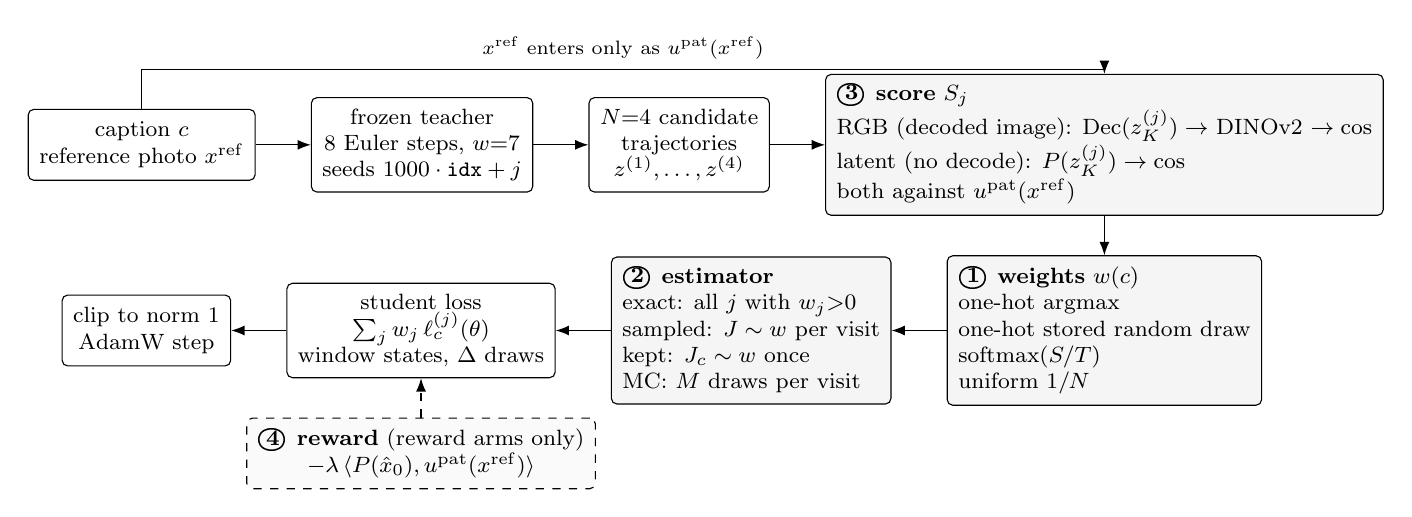
\begin{tikzpicture}[
  node distance=5mm and 7mm, >=Latex, font=\footnotesize,
  box/.style={draw, rounded corners=2pt, align=center, inner sep=4pt, minimum height=9mm},
  choice/.style={draw, rounded corners=2pt, align=left, inner sep=4pt, fill=black!4},
  opt/.style={draw, dashed, rounded corners=2pt, align=center, inner sep=4pt, fill=black!2},
  lab/.style={font=\bfseries\footnotesize, fill=white, inner sep=1pt}]
\node[box] (cap) {caption $c$\\ reference photo $x^{\mathrm{ref}}$};
\node[box, right=of cap] (tea) {frozen teacher\\ 8 Euler steps, $w{=}7$\\ seeds $1000\cdot\texttt{idx}+j$};
\node[box, right=of tea] (cand) {$N{=}4$ candidate\\ trajectories\\ $z^{(1)},\dots,z^{(4)}$};
\node[choice, right=of cand] (score) {\textbf{\textcircled{3} score} $S_j$\\ RGB (decoded image): $\Dec(z_K^{(j)})\to$ DINOv2 $\to\cos$\\ latent (no decode): $P(z_K^{(j)})\to\cos$\\ both against $u^{\mathrm{pat}}(x^{\mathrm{ref}})$};
\node[choice, below=of score] (w) {\textbf{\textcircled{1} weights} $w(c)$\\ one-hot argmax\\ one-hot stored random draw\\ softmax$(S/T)$\\ uniform $1/N$};
\node[choice, left=of w] (est) {\textbf{\textcircled{2} estimator}\\ exact: all $j$ with $w_j{>}0$\\ sampled: $J\sim w$ per visit\\ kept: $J_c\sim w$ once\\ MC: $M$ draws per visit};
\node[box, left=of est] (loss) {student loss\\ $\sum_j w_j\,\ell_c^{(j)}(\theta)$\\ window states, $\Delta$ draws};
\node[box, left=of loss] (step) {clip to norm 1\\ AdamW step};
\node[opt, below=of loss] (rew) {\textbf{\textcircled{4} reward} (reward arms only)\\ $-\lambda\,\langle P(\hat{x}_0),u^{\mathrm{pat}}(x^{\mathrm{ref}})\rangle$};
\draw[->] (cap) -- (tea); \draw[->] (tea) -- (cand); \draw[->] (cand) -- (score);
\draw[->] (score) -- (w); \draw[->] (w) -- (est); \draw[->] (est) -- (loss); \draw[->] (loss) -- (step);
\draw[->, dashed] (rew) -- (loss);
\draw[->] (cap.north) -- ++(0,5mm) -| node[pos=0.25, above, font=\scriptsize]{$x^{\mathrm{ref}}$ enters only as $u^{\mathrm{pat}}(x^{\mathrm{ref}})$} (score.north);
\end{tikzpicture}
\caption{One training update. Every arm follows this flow; the four numbered blocks are the only places where arms differ (Table~\ref{tab:arms}). The reference photograph enters only through its DINOv2 embedding, in the score and, in the reward arms, in the reward.}
\label{fig:pipeline}
\end{figure}

\begin{itemize}
\item \textbf{\textcircled{1} The weights $w(c)$ over the candidates.} A function of a per-candidate score $S_j(c)$ and a temperature $T$:
  \begin{itemize}
  \item \emph{argmax}: $w_j=\mathbb{1}[j=\argmax_l S_l]$ (the method);
  \item \emph{random}: $w_j=\mathbb{1}[j=J_c]$ with $J_c\sim\mathcal{U}\{1..N\}$ drawn once and stored in the cache (the baseline);
  \item \emph{Boltzmann}: $w_j=\pi_j=\exp(S_j/T)\big/\sum_l\exp(S_l/T)$, on the raw score scale;
  \item \emph{uniform}: $w_j=1/N$ (the $T\to\infty$ limit; no selection).
  \end{itemize}
\item \textbf{\textcircled{2} The estimator of the weighted sum $\sum_jw_j\ell^{(j)}$.} For one-hot weights all four coincide.
  \begin{itemize}
  \item \emph{exact}: every candidate with $w_j>0$ is rolled out and its loss weighted by $w_j$; cost proportional to the number of candidates;
  \item \emph{sampled}: one index $J\sim w$ is drawn on each visit of the caption and $\ell^{(J)}$ is used; single-candidate cost, the same expected gradient, different optimizer updates (Section~\ref{sec:graddiag});
  \item \emph{kept}: $J_c\sim w$ is drawn once per caption and reused on every visit (the persistence control);
  \item \emph{same-caption Monte Carlo}: $M$ independent draws per visit, losses weighted by their counts over $M$ (implemented, not run).
  \end{itemize}
\item \textbf{\textcircled{3} The score $S_j$.} Both use the reference photograph only through its DINOv2 patch-mean embedding $u^{\mathrm{pat}}(x^{\mathrm{ref}})$:
  \begin{itemize}
  \item \emph{RGB}, the decoded-image scorer of Section~\ref{sec:scorers}, named for reading the decoded RGB image: $S_j=\big\langle u^{\mathrm{pat}}(\Dec(z_K^{(j)})),\,u^{\mathrm{pat}}(x^{\mathrm{ref}})\big\rangle$, the candidate decoded and embedded with DINOv2;
  \item \emph{latent} (Section~\ref{sec:latent}): $\hat S_j=\big\langle P(z_K^{(j)}),\,u^{\mathrm{pat}}(x^{\mathrm{ref}})\big\rangle$, the candidate's terminal latent mapped into the same space by the projector $P$, no decode;
  \item VQAScore, DINOv2 CLS, CLIP-I, ImageReward and PickScore (Table~\ref{tab:headroom}) are further choices of $S$, used with argmax only.
  \end{itemize}
\item \textbf{\textcircled{4} The reward $r_c(\theta)$} (Section~\ref{sec:reward}; $\lambda=0$ everywhere else):
  \begin{itemize}
  \item $r_c(\theta)=\frac{1}{R}\sum_{s\in\mathcal{R}}\big\langle P(\hat{x}_0(z^{(J)}_s;\theta)),\,u^{\mathrm{pat}}(x^{\mathrm{ref}})\big\rangle$ on the student's own clean estimates from the $R=2$ least-noisy supervised inputs, with the gradient flowing through $P$ into the student;
  \item \emph{frozen}: $P$ is the offline projector throughout;
  \item \emph{refreshed}: every 100 updates $P$ takes four steps toward the RGB scorer on decoded recent predictions, with replay of teacher candidates (Figure~\ref{fig:rewardloop}).
  \end{itemize}
\end{itemize}

\begin{figure}[H]
\centering
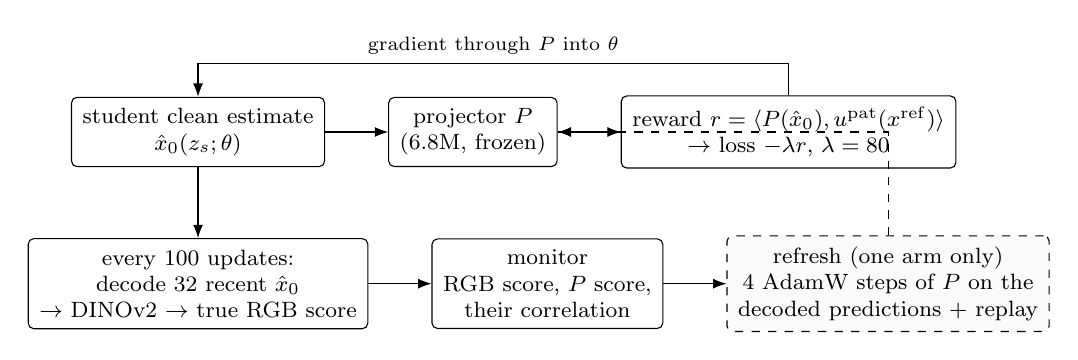
\begin{tikzpicture}[node distance=5mm and 8mm, >=Latex, font=\footnotesize,
  box/.style={draw, rounded corners=2pt, align=center, inner sep=4pt, minimum height=8mm},
  opt/.style={draw, dashed, rounded corners=2pt, align=center, inner sep=4pt, fill=black!2}]
\node[box] (xh) {student clean estimate\\ $\hat{x}_0(z_s;\theta)$};
\node[box, right=of xh] (P) {projector $P$\\ (6.8M, frozen)};
\node[box, right=of P] (r) {reward $r=\langle P(\hat{x}_0),u^{\mathrm{pat}}(x^{\mathrm{ref}})\rangle$\\ $\to$ loss $-\lambda r$, $\lambda=80$};
\node[box, below=9mm of xh] (dec) {every 100 updates:\\ decode 32 recent $\hat{x}_0$\\ $\to$ DINOv2 $\to$ true RGB score};
\node[box, right=of dec] (mon) {monitor\\ RGB score, $P$ score,\\ their correlation};
\node[opt, right=of mon] (ref) {refresh (one arm only)\\ 4 AdamW steps of $P$ on the\\ decoded predictions + replay};
\draw[->] (xh) -- (P); \draw[->] (P) -- (r);
\draw[->] (r.north) -- ++(0,4mm) -| node[pos=0.25, above, font=\scriptsize]{gradient through $P$ into $\theta$} (xh.north);
\draw[->] (xh) -- (dec); \draw[->] (dec) -- (mon); \draw[->] (mon) -- (ref);
\draw[->, dashed] (ref.north) |- (P.east);
\end{tikzpicture}
\caption{The reward arms of Section~\ref{sec:reward}. Solid: the reward path used on every update. Below: the hacking monitor that decodes recent predictions and scores them with the RGB scorer, and, in the refreshed arm, the projector update it feeds.}
\label{fig:rewardloop}
\end{figure}
Two further terms appear only in the ablations and are written where they are used: the real-photograph regression (Section~\ref{sec:ablations}) adds a pseudo-Huber term between $\hat{x}_0$ and the VAE latent of $x^{\mathrm{ref}}$; the evolving-teacher variant replaces the frozen teacher in $z^{(j)}$ and $\tilde{x}_0$ by an EMA copy of the student.

\subsection{Every arm against the four choices}
Table~\ref{tab:arms} lists every arm as its choice of weights, estimator, score and reward.
\begin{table}[H]
\centering
\caption{The arms of this document. Cost is teacher rollouts and student passes per caption per update relative to the random arm (1 rollout, $K_w=5$ student passes). Where an arm appears is given by section.}
\label{tab:arms}
\footnotesize\setlength{\tabcolsep}{3pt}
\begin{tabular}{>{\raggedright\arraybackslash}p{2.9cm} >{\raggedright\arraybackslash}p{2.3cm} >{\raggedright\arraybackslash}p{1.8cm} >{\raggedright\arraybackslash}p{2.4cm} >{\raggedright\arraybackslash}p{2.3cm} >{\centering\arraybackslash}p{0.8cm} >{\raggedright\arraybackslash}p{2.0cm}}
\toprule
Arm (name in tables) & weights $w$ & estimator & score $S$ & reward & cost & where \\
\midrule
random (fixed draw) & one-hot, stored uniform draw & -- & -- & -- & 1 & everywhere (baseline) \\
argmax (DINOv2 patches) & one-hot on $\argmax S$ & -- & RGB DINO patch & -- & 1 & everywhere (the method) \\
argmax, other scorer & one-hot on $\argmax S$ & -- & VQAScore, CLS, CLIP-I, ImageReward, PickScore & -- & 1 & Sections~\ref{sec:main}, \ref{sec:scale} \\
\midrule
Boltzmann $T$, exact & $\pi_j=\mathrm{softmax}(S/T)$ & exact & RGB DINO patch & -- & 4 & Section~\ref{sec:selrule} \\
uniform, exact & $1/N$ & exact & -- & -- & 4 & Section~\ref{sec:selrule} \\
Boltzmann $T$, sampled & $\pi_j$ & sampled per visit & RGB DINO patch & -- & 1 & Section~\ref{sec:selrule} \\
uniform, redrawn per visit & $1/N$ & sampled per visit & -- & -- & 1 & Section~\ref{sec:selrule} \\
Boltzmann $T$, one draw kept & $\pi_j$ & kept per caption & RGB DINO patch & -- & 1 & Section~\ref{sec:selrule} \\
same-caption MC, $M$ draws & $\pi_j$ & counts$/M$ per visit & RGB DINO patch & -- & $\le4$ & implemented, not run \\
\midrule
argmax, latent scorer & one-hot on $\argmax\hat S$ & -- & latent projector & -- & 1 & Section~\ref{sec:latent} \\
Boltzmann $T$ exact, latent scorer & $\mathrm{softmax}(\hat S/T)$ & exact & latent projector & -- & 4 & Section~\ref{sec:latent} \\
\midrule
argmax + projector reward, frozen & one-hot on $\argmax S$ & -- & RGB DINO patch & $\lambda=80$, $R=2$, $P$ frozen & 1 (+$P$) & Section~\ref{sec:reward} \\
argmax + projector reward, refreshed & one-hot on $\argmax S$ & -- & RGB DINO patch & $\lambda=80$, $R=2$, $P$ refreshed & 1 (+$P$) & Section~\ref{sec:reward} \\
\midrule
118k arms; $N=8$; batch 16 & as above & -- & as above & -- & 1 & Section~\ref{sec:scale} \\
16-step / 28-step teacher & one-hot & -- & RGB DINO patch & -- & 1 & Section~\ref{sec:k28} \\
+ real-photograph term & one-hot & -- & RGB DINO patch & pseudo-Huber to the photo latent & 1 & Section~\ref{sec:ablations} \\
evolving (EMA) teacher & one-hot on online $S$ & -- & RGB DINO patch, online & -- & 4 (+decode) & Section~\ref{sec:ema} \\
\bottomrule
\end{tabular}
\end{table}

\subsection{The networks}
Table~\ref{tab:networks} lists the networks involved, their sizes and roles, and which of them train.
\begin{table}[H]
\centering
\caption{Every network in the pipeline, what it does, and whether it trains.}
\label{tab:networks}
\footnotesize\setlength{\tabcolsep}{4pt}
\begin{tabular}{>{\raggedright\arraybackslash}p{2.0cm} >{\raggedright\arraybackslash}p{4.9cm} >{\raggedright\arraybackslash}p{4.3cm} >{\raggedright\arraybackslash}p{3.8cm}}
\toprule
Network & Architecture and size & Role & Trained? \\
\midrule
Teacher & SD3.5-Medium MMDiT, 2.5B, bf16 & candidate rollouts ($K=8$, $w=7$) and targets $\tilde{x}_0$ & no (frozen); EMA copy of the student in Section~\ref{sec:ema} only \\
Student & same MMDiT, initialised from the teacher, fp32 master weights & $\hat{x}_0$ at the supervised states; sampled at 4 steps, $w=1$ & yes (the only network trained in the main method) \\
Text encoders & CLIP-L, CLIP-G, T5-XXL & caption conditioning of both & no \\
VAE & SD3.5 VAE & decode candidates for scoring; decode for evaluation & no \\
RGB scorer & DINOv2-B, 86M; patch-mean, CLS dropped, L2-normalised & $S_j$ (offline) & no \\
Latent projector $P$ & 5-stage conv encoder (64, 128, 256, 512, 512; GN, SiLU), global mean pool, MLP 512--1024--768, L2-normalised; 6.8M & $\hat S_j$ (offline) and the reward $r_c$ & once, offline, on 22k held-out captions (5 min); refreshed during training in one reward arm \\
\bottomrule
\end{tabular}
\end{table}

\subsection{The projector's three settings, in the order they were tried}
The latent projector $P$ appears in three settings that build on each other; Table~\ref{tab:projector_uses} lists them in order, with the check that sits between the second and the first.

\begin{table}[H]
\centering
\caption{The three uses of the latent projector $P$. In every setting $P$ is first trained once, offline, on 22,000 held-out captions (five minutes); the settings differ in what it scores and whether it moves afterwards.}
\label{tab:projector_uses}
\footnotesize\setlength{\tabcolsep}{4pt}
\begin{tabular}{>{\raggedright\arraybackslash}p{0.6cm} >{\raggedright\arraybackslash}p{2.9cm} >{\raggedright\arraybackslash}p{3.3cm} >{\raggedright\arraybackslash}p{2.8cm} >{\raggedright\arraybackslash}p{4.2cm}}
\toprule
 & setting & what $P$ scores, when & arms & outcome \\
\midrule
1 & \textbf{offline selector, frozen} (Section~\ref{sec:latent}) & the cached teacher candidates $z_K^{(j)}$, once before training; the score goes into the cache and the trainer is unchanged & argmax, latent scorer; Boltzmann $T{=}0.04$ exact, latent scorer & recovers 34\% of the VQAScore headroom (RGB: 44\%); trained students $0.003$ below their RGB counterparts, identical fidelity \\
\addlinespace
-- & \textbf{transfer check} (Section~\ref{sec:latent}, R0) & the students' own 4-step samples, offline & none (diagnostic) & agreement with the RGB scorer drops (top-1 0.51 $\to$ 0.37); fine-tuning on 1,000 student latents does not restore it \\
\addlinespace
2 & \textbf{in-loop reward, frozen} (Section~\ref{sec:reward}) & the student's clean estimates $\hat{x}_0$ at the two least-noisy supervised inputs, on every update; $-\lambda r$ added to the loss, $\lambda=80$ & argmax + projector reward, frozen & reward rises 0.03; true RGB score of the same predictions does not; CompBench $-0.003\pm0.005$ vs argmax \\
\addlinespace
3 & \textbf{in-loop reward, refreshed} (Section~\ref{sec:reward}) & as 2, and every 100 updates $P$ takes four steps toward the RGB scorer on 32 decoded recent predictions, with replay of teacher candidates & argmax + projector reward, refreshed & reward rises 0.04; RGB score flat; agreement with the RGB scorer 0.41 vs 0.36 frozen; CompBench $+0.000\pm0.008$ vs argmax \\
\bottomrule
\end{tabular}
\end{table}

\subsection{How to read the comparisons}
Figure~\ref{fig:allarms} places every 3k-pool arm on one axis, Figure~\ref{fig:contrasts} shows each arm's seed-paired difference to argmax, Figure~\ref{fig:rawavg} shows what checkpoint averaging does to each arm, and Figure~\ref{fig:heatmap} shows where in CompBench the differences sit. Each results table in Sections~\ref{sec:main} to~\ref{sec:selrule} changes one row of Table~\ref{tab:arms} at a time.

\begin{figure}[p]
\centering
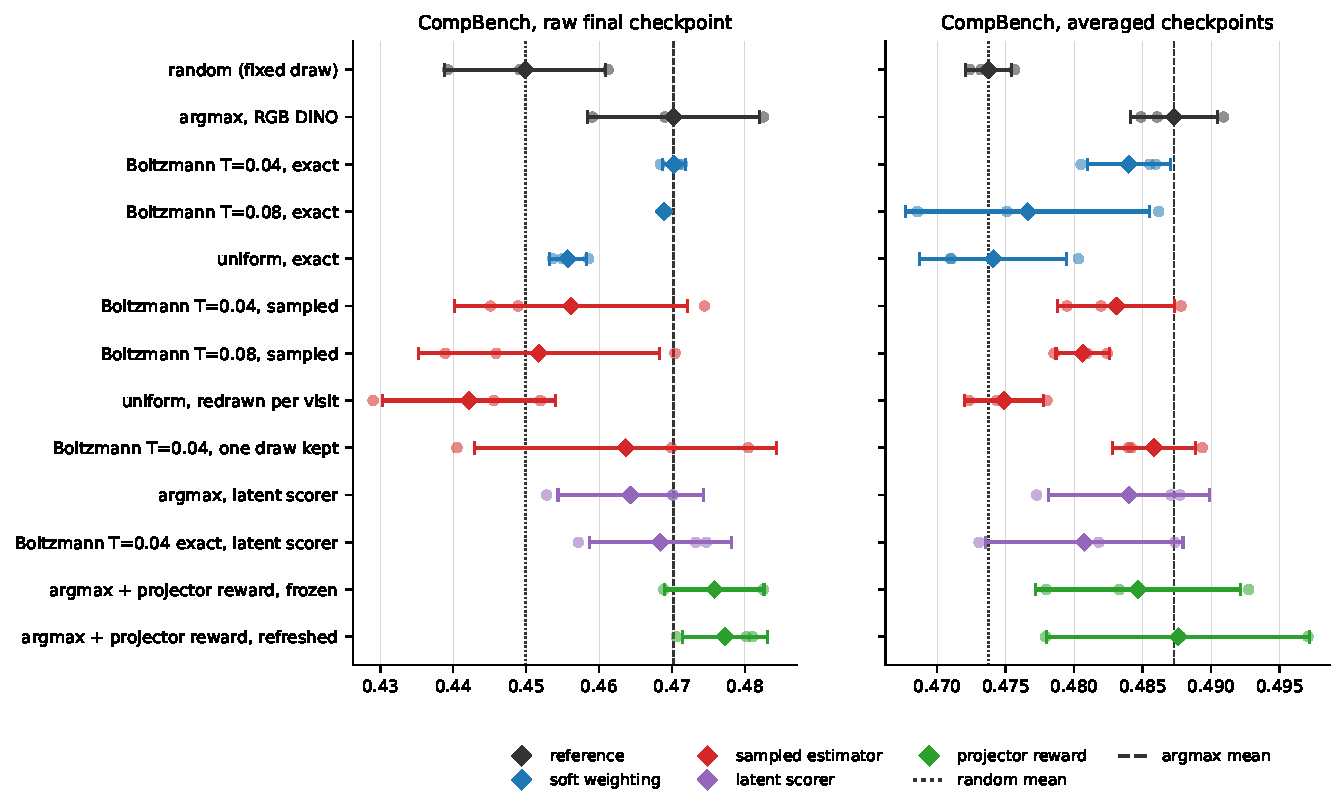
\includegraphics[width=0.9\textwidth]{figs/all_arms_compbench.pdf}
\caption{All arms trained on the 3k pool with the 3k configuration, three seeds each: CompBench seed values (dots), mean and standard deviation (diamond, bar), on raw final and on averaged checkpoints. Dotted and dashed lines are the random and argmax means. Colours group the arms by the choice they vary in Table~\ref{tab:arms}.}
\label{fig:allarms}
\end{figure}

\begin{figure}[p]
\centering
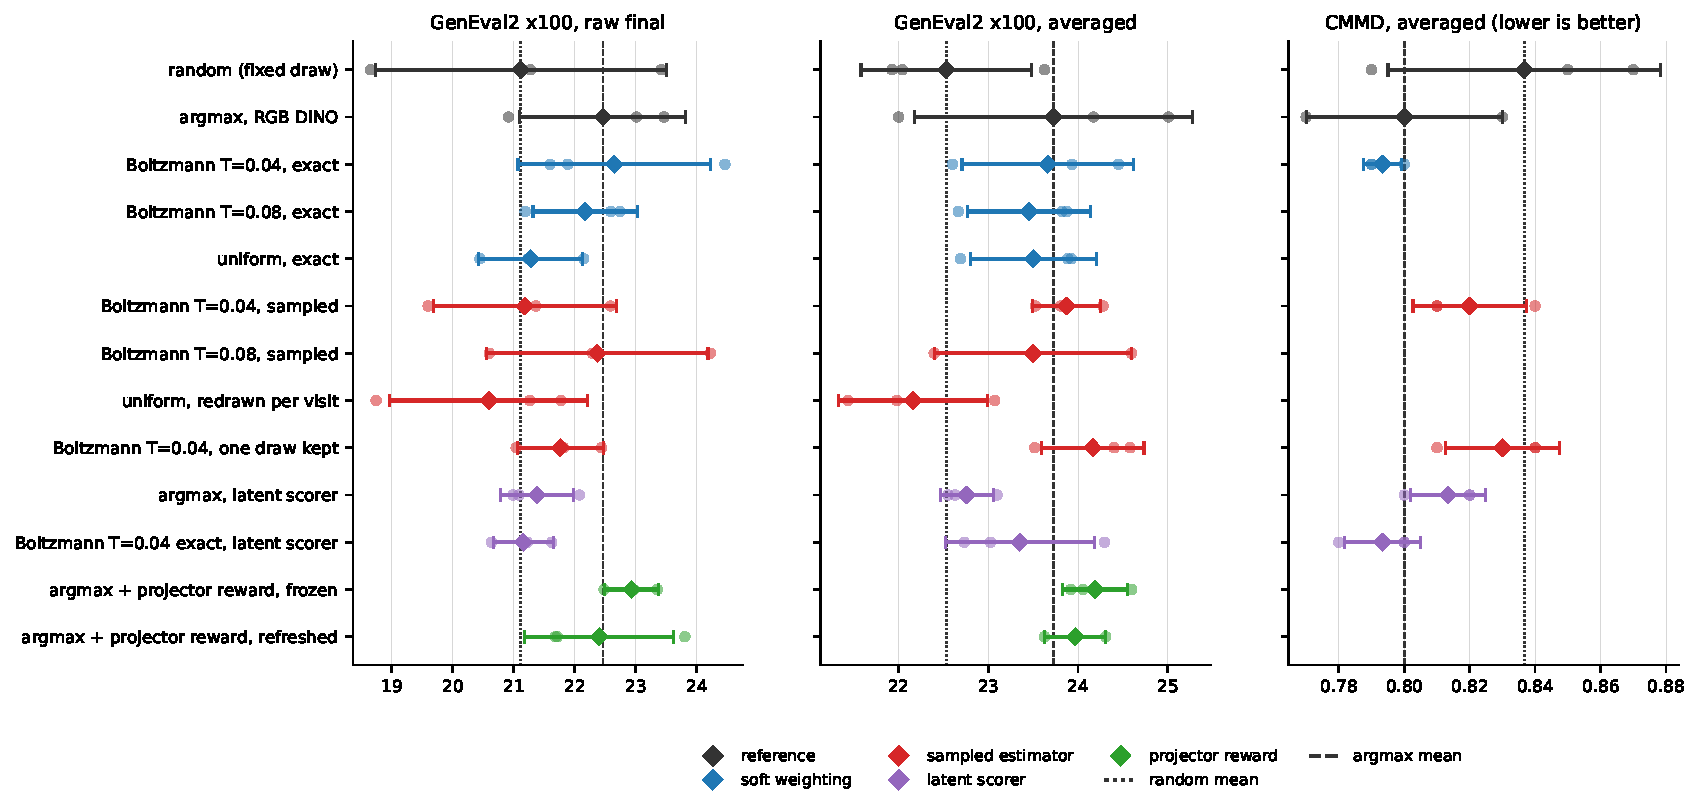
\includegraphics[width=\textwidth]{figs/all_arms_other.pdf}
\caption{The same arms on GenEval2 (raw final and averaged checkpoints) and on CMMD (averaged checkpoints, lower is better). GenEval2 does not separate any two arms at three seeds; CMMD is within 0.03 for every scored arm after averaging.}
\label{fig:allarms2}
\end{figure}

\begin{figure}[p]
\centering
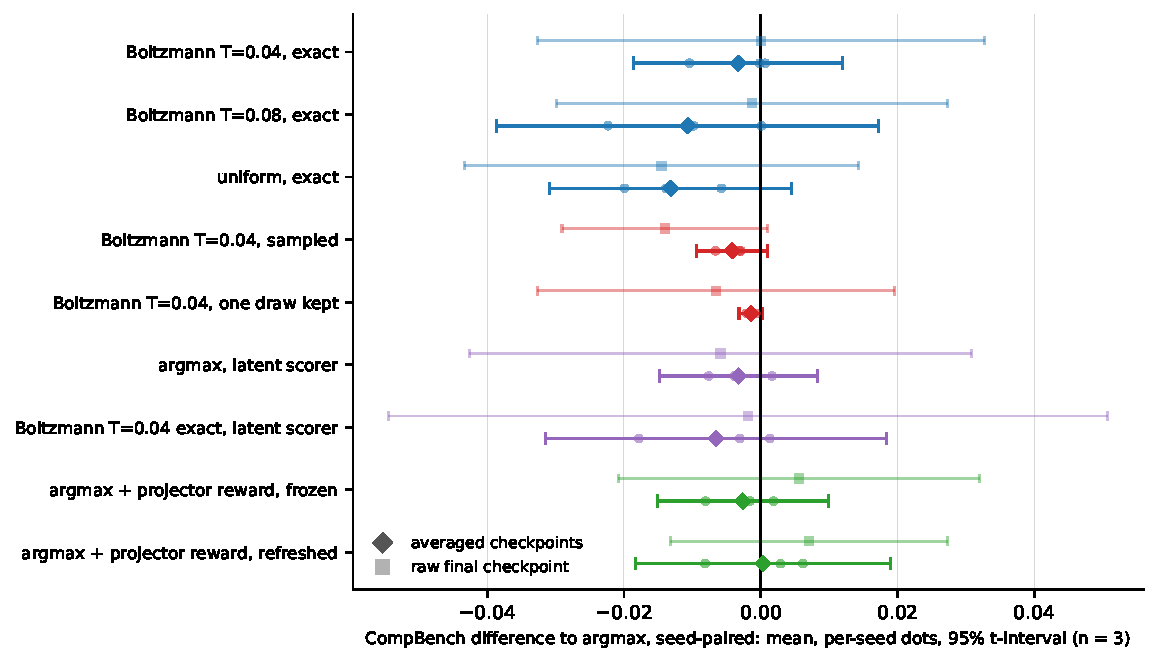
\includegraphics[width=0.85\textwidth]{figs/contrasts.pdf}
\caption{Seed-paired CompBench difference of every arm to argmax on averaged checkpoints (diamonds, with per-seed dots and 95\% $t$-intervals) and on raw final checkpoints (faint squares). Intervals that cross zero are ``no detected difference''; three seeds resolve about 0.01.}
\label{fig:contrasts}
\end{figure}

\begin{figure}[ht]
\centering
\begin{minipage}[t]{0.42\textwidth}
\centering
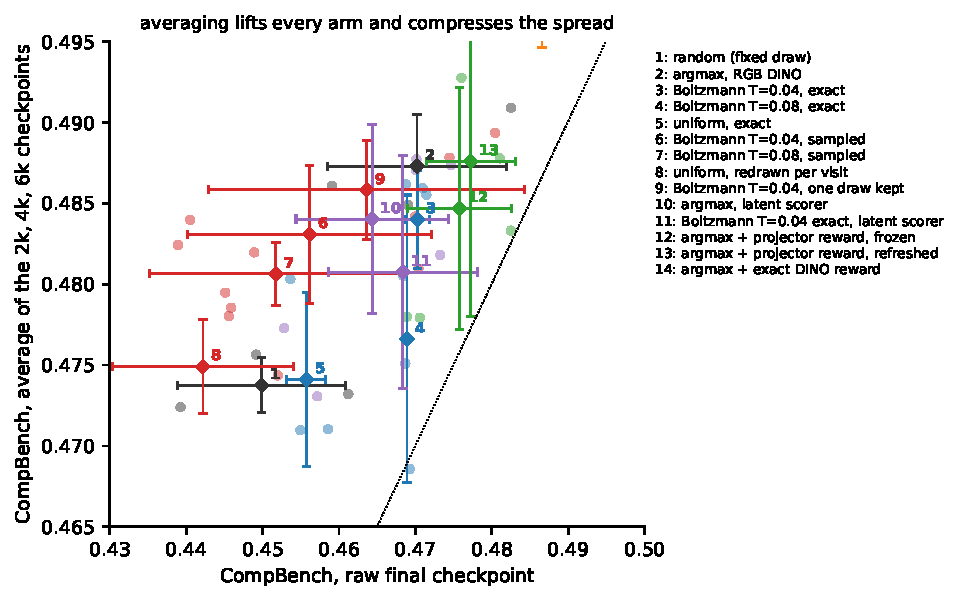
\includegraphics[width=\textwidth]{figs/raw_vs_avg.pdf}
\caption{Raw final against averaged CompBench per arm. Averaging lifts every arm by 0.01 to 0.03 and shrinks the differences between them; the arms that gain most are those whose final iterate wanders most.}
\label{fig:rawavg}
\end{minipage}\hfill
\begin{minipage}[t]{0.56\textwidth}
\centering
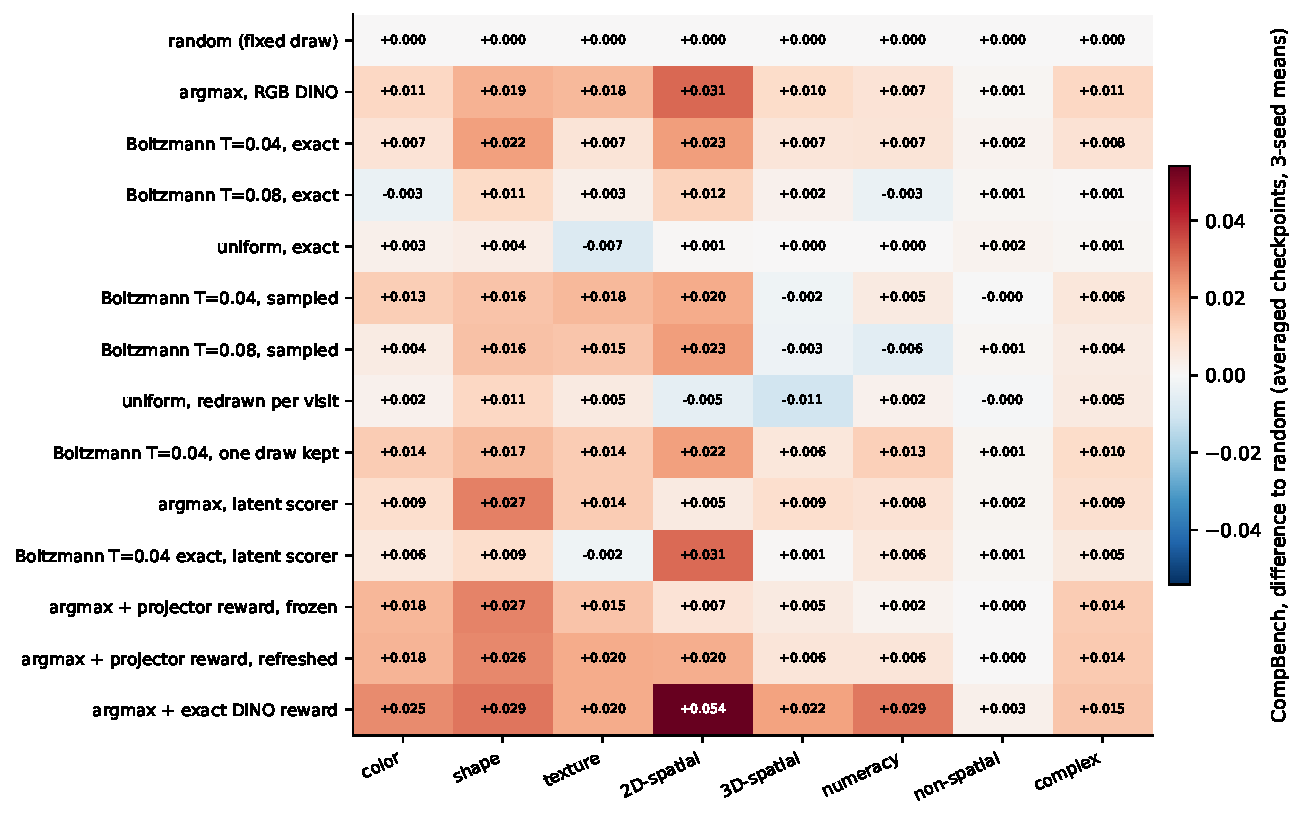
\includegraphics[width=\textwidth]{figs/category_heatmap.pdf}
\caption{CompBench per category, averaged checkpoints, three-seed means, as differences to the random arm. The scored arms gain on colour, shape, spatial and numeracy and not on non-spatial, whose CLIPScore evaluator does not separate students.}
\label{fig:heatmap}
\end{minipage}
\end{figure}

\section{Evaluation}

\subsection{Alignment}
\begin{itemize}
\item \textbf{T2I-CompBench.} 2,398 prompts, official scorers: BLIP-VQA for color, shape and texture; UniDet for 2D-spatial, 3D-spatial and numeracy; CLIPScore for non-spatial; the 3-in-1 score for complex. The overall score is the unweighted mean of the eight category means. One image per prompt, seed equal to the prompt index, so every arm sees identical noise.
\item \textbf{GenEval2.} 800 prompts. Each prompt is decomposed into 3 to 10 atoms tagged object, count, attribute, position or verb. Qwen3-VL scores each atom with a probability (Soft-TIFA). The prompt score is the geometric mean of its atom scores, and the official number is the mean prompt score $\times100$.
\item \textbf{COCO VQAScore.} 5,000 held-out \texttt{val2017} captions scored by VQAScore. This is in-domain for the training captions. For the VQAScore-selected arm this metric is circular.
\end{itemize}

\subsection{Fidelity}
5,000 images from \texttt{val2017} captions against the 5,000 matching real photographs, centre-cropped to squares. FID uses clean-fid. CMMD uses the reference implementation: CLIP ViT-L/14 at 336 px, centre crop then bicubic resize, unit-normalised embeddings, RBF kernel with $\sigma=10$, biased estimator, $\times1000$. Precision and recall use $k$-NN manifolds. CMMD intervals are 1,000-sample bootstraps.

\subsection{Statistics}
Deltas are paired on identical prompts. For the three-seed experiments on the 3k pool, the interval is a hierarchical bootstrap that resamples seeds and prompts jointly (4,000 resamples). The 118k and selection-rule contrasts report per-prompt paired $t$-tests (Wilcoxon tests agree throughout), pooled over seeds where there are several, with the per-seed deltas alongside.

\subsection{Two properties of the metrics that matter for reading the tables}
\label{sec:metricprops}
\paragraph{GenEval2 rewards partial credit.}
On the geometric-mean score the 28-step teacher (17.05) scores below every 4-step student (20.7 to 23.7). On strict accuracy, the share of prompts with every atom above 0.5, the teacher leads (10.2\% against 6.7 to 8.2\%), and it leads on the arithmetic atom mean, on CompBench and on COCO VQAScore. The reason is that the judge gives the teacher's wrong atoms probabilities near zero, while the students' wrong atoms, mostly attribute and position atoms, get mid-range probabilities. One near-zero atom sends a geometric mean to zero, so 61\% of the teacher's prompts collapse against 35 to 39\% for the students, although both fail about 2.3 atoms per prompt. GenEval2 scores should therefore be read as relative numbers between students, not as evidence that a student beats the teacher.

\paragraph{CompBench 2D-spatial has dead prompts.}
The official 2D-spatial evaluator matches prompt nouns to detector labels by exact string equality. 31.8\% of the official spatial prompts, and 98 of our 298, contain a noun that no label matches (for example \emph{cow}, \emph{sofa}, \emph{wallet}), and they score zero for every possible image. This scales the spatial column by a constant and does not reorder models (rank correlation 0.91 between official and repaired scoring, no significant reversal). Spatial deltas are therefore understated by about $1.5\times$ relative to other categories.

\section{Results on the 3k pool}
\label{sec:main}

\subsection{Alignment, all scorers}
Table~\ref{tab:main3k} is the main result. Every arm is three seeds on the same 3k pool, the same candidate cache and the same configuration.

\begin{table}[ht]
\centering
\caption{3k pool, 6,000 updates, three seeds. Absolute scores are seed means. Deltas are against the random-selection student with 95\% hierarchical bootstrap intervals. Bold intervals exclude zero.}
\label{tab:main3k}
\resizebox{\textwidth}{!}{%
\begin{tabular}{l l c c c c c}
\toprule
Scorer & Needs & CompBench & CompBench $\Delta$ & GenEval2 & GenEval2 $\Delta$ ($\times100$) & COCO VQAScore \\
\midrule
random (baseline) & -- & 0.4584 & -- & 20.73 & -- & 0.8733 \\
DINOv2 patches & photo & 0.4725 & \textbf{+0.0140 [+0.0051, +0.0237]} & 22.89 & \textbf{+2.17 [+0.24, +4.08]} & 0.8850 \\
DINOv2 CLS & photo & 0.4620 & +0.0036 [$-$0.0062, +0.0142] & 21.73 & +1.00 [$-$0.80, +2.86] & 0.8799 \\
CLIP-I & photo & 0.4595 & +0.0010 [$-$0.0112, +0.0130] & 21.23 & +0.51 [$-$1.44, +2.49] & 0.8748 \\
VQAScore & caption & 0.4817 & \textbf{+0.0233 [+0.0097, +0.0364]} & 23.06 & \textbf{+2.34 [+0.55, +4.05]} & 0.8873 \\
ImageReward & caption & 0.4806 & \textbf{+0.0221 [+0.0127, +0.0322]} & 22.17 & +1.45 [$-$0.43, +3.37] & 0.8854 \\
PickScore & caption & 0.4713 & \textbf{+0.0128 [+0.0012, +0.0245]} & 22.52 & +1.80 [$-$0.05, +3.72] & 0.8850 \\
\midrule
Teacher, 8 steps, $w=7$ (source) & & 0.4544 & & 17.58 & & -- \\
Teacher, 28 steps, $w=7$ & & 0.5053 & & 17.05 & & 0.9102 \\
Base model, 4 steps, $w=7$ & & 0.2557 & & 7.32 & & 0.4762 \\
\bottomrule
\end{tabular}}
\end{table}

Three points follow from the table.
\begin{itemize}
\item The DINOv2 patch scorer, which reads no text, recovers 60\% of VQAScore's CompBench gain and 93\% of its GenEval2 gain.
\item Mean-pooled patches beat the CLS token. Head-to-head on identical prompts the patch arm is ahead of the CLS arm by $+0.0104$ CompBench ($p=10^{-5}$), $+0.0108$ on UniDet, $+0.0154$ on BLIP-VQA and $+1.17$ GenEval2, positive on all three seeds for every endpoint. CLIP-I, the other reference-photo scorer, is a null.
\item Every 4-step student beats the 8-step teacher it was distilled from on CompBench. The 28-step teacher remains clearly better on CompBench and COCO VQAScore. Its lower GenEval2 number is the metric property of Section~\ref{sec:metricprops}.
\end{itemize}

\subsection{Fidelity}
Table~\ref{tab:fid3k} shows that scored selection does not cost fidelity. Every scored arm has lower CMMD than the random baseline, and precision and recall are equal or higher. FID differences between students are within the split-half spread of about 0.5 and should not be read.

\begin{table}[ht]
\centering
\caption{Fidelity on 5,000 COCO \texttt{val2017} captions, 4 steps, $w=1$, seed means over three runs. CMMD bootstrap intervals are about $\pm0.01$.}
\label{tab:fid3k}
\begin{tabular}{l c c c c}
\toprule
Arm & FID $\downarrow$ & CMMD $\downarrow$ & Precision $\uparrow$ & Recall $\uparrow$ \\
\midrule
random (baseline) & 32.64 & 0.963 & 0.440 & 0.041 \\
DINOv2 patches & 30.72 & 0.893 & 0.465 & 0.052 \\
DINOv2 CLS & 30.98 & 0.913 & 0.467 & 0.046 \\
CLIP-I & 32.45 & 0.870 & 0.484 & 0.049 \\
VQAScore & 30.97 & 0.883 & 0.461 & 0.052 \\
ImageReward & 30.71 & 0.867 & 0.470 & 0.056 \\
PickScore & 31.02 & 0.907 & 0.444 & 0.049 \\
\midrule
Teacher, 28 steps, $w=7$ & 29.21 & 0.640 & 0.549 & 0.156 \\
Base model, 4 steps, $w=7$ & 94.48 & 2.150 & 0.178 & 0.006 \\
\bottomrule
\end{tabular}
\end{table}

\subsection{Absolute scores per category}
Tables~\ref{tab:geneval2_skills} to~\ref{tab:compbench_categories} give per-category absolute scores for the teacher, the base model and the four main arms. The largest per-skill gain of the DINOv2 patch scorer on GenEval2 is on \emph{position} (51.4 against 45.9), consistent with mean-pooled patches carrying layout, and its advantage grows with prompt complexity.

\begin{table}[ht]
\centering
\caption{GenEval2 (Soft-TIFA, Qwen3-VL judge), $\times 100$, on the sealed 800-prompt pool. \emph{Overall} is the official score, the mean over prompts of the geometric mean of a prompt's atom scores ($\pm$ standard deviation over training seeds). Skill columns are the mean score of the atoms tagged with that skill. \emph{Atom mean} is the arithmetic mean over all atoms. \emph{Collapsed} is the share of prompts whose geometric mean falls below 0.05. Teacher and base rows are single deterministic runs. Bold marks the best 4-step distilled arm in each column.}
\label{tab:geneval2_skills}
\resizebox{\textwidth}{!}{%
\begin{tabular}{l c c c ccccc c c}
\toprule
Model & Steps / CFG & Seeds & Overall & Object & Count & Attribute & Position & Verb & Atom mean & Collapsed (\%) \\
\midrule
Teacher, 28 steps, CFG 7 & 28 / 7 & 1 & 17.05 & 87.6 & 44.7 & 66.1 & 45.7 & 17.4 & 64.7 & 60.6 \\
Teacher, 8 steps, CFG 7 (source) & 8 / 7 & 1 & 17.58 & 83.7 & 40.6 & 67.5 & 42.5 & 18.3 & 62.1 & 54.8 \\
Base, 4 steps, CFG 7 & 4 / 7 & 1 & 7.32 & 43.2 & 20.8 & 49.9 & 26.9 & 4.4 & 36.2 & 79.0 \\
\midrule
Naive CD (random pick) & 4 / 1 & 3 & 20.73 $\pm$ 0.94 & 80.5 & 34.8 & 69.5 & 45.9 & 21.4 & 59.8 & 38.5 \\
Scored CD, DINO CLS & 4 / 1 & 3 & 21.73 $\pm$ 0.76 & 82.7 & 34.4 & 70.1 & 48.5 & 24.2 & 60.9 & 37.0 \\
Scored CD, DINO patches & 4 / 1 & 3 & 22.89 $\pm$ 1.01 & 82.8 & 34.6 & 70.5 & \textbf{51.4} & 26.0 & 61.4 & 35.4 \\
Scored CD, VQAScore & 4 / 1 & 3 & \textbf{23.06 $\pm$ 0.15} & \textbf{84.3} & \textbf{35.6} & \textbf{70.7} & 47.8 & \textbf{26.6} & \textbf{62.1} & \textbf{34.8} \\
\bottomrule
\end{tabular}}
\end{table}

\begin{table}[ht]
\centering
\caption{GenEval2 by prompt complexity: mean prompt score ($\times 100$) in each atom-count bucket, 100 prompts per bucket, averaged over training seeds where applicable. Bold marks the best 4-step distilled arm in each column.}
\label{tab:geneval2_complexity}
\begin{tabular}{l cccccccc}
\toprule
Model & 3 & 4 & 5 & 6 & 7 & 8 & 9 & 10 \\
\midrule
Teacher, 28 steps, CFG 7 & 36.3 & 32.5 & 22.5 & 19.9 & 12.8 & 4.7 & 5.5 & 2.3 \\
Teacher, 8 steps, CFG 7 (source) & 34.2 & 35.6 & 23.2 & 18.1 & 11.2 & 9.0 & 4.9 & 4.2 \\
Base, 4 steps, CFG 7 & 21.0 & 8.3 & 8.7 & 6.9 & 3.9 & 4.7 & 3.0 & 2.1 \\
\midrule
Naive CD (random pick) & 38.9 & 34.2 & 22.8 & 20.9 & 15.9 & 13.6 & 11.7 & 7.8 \\
Scored CD, DINO CLS & 43.2 & 34.2 & 24.4 & 22.2 & 15.5 & 13.7 & 13.0 & 7.5 \\
Scored CD, DINO patches & 41.6 & \textbf{35.6} & \textbf{25.4} & \textbf{24.7} & \textbf{17.7} & \textbf{15.3} & \textbf{14.3} & 8.6 \\
Scored CD, VQAScore & \textbf{48.4} & 33.4 & 24.6 & 24.1 & 17.3 & 14.0 & 13.2 & \textbf{9.4} \\
\bottomrule
\end{tabular}
\end{table}

\begin{table}[ht]
\centering
\caption{T2I-CompBench on the sealed 2{,}398-prompt pool, official scorers, one image per prompt. \emph{Mean} is the unweighted mean of the eight categories ($\pm$ standard deviation over training seeds); category columns are averaged over seeds. Bold marks the best 4-step distilled arm in each column.}
\label{tab:compbench_categories}
\resizebox{\textwidth}{!}{%
\begin{tabular}{l c cccccccc}
\toprule
Model & Mean & Color & Shape & Texture & Spatial & 3D-spatial & Numeracy & Non-spatial & Complex \\
\midrule
Teacher, 28 steps, CFG 7 & 0.5053 & 0.7977 & 0.5732 & 0.7427 & 0.2716 & 0.3662 & 0.5915 & 0.3154 & 0.3837 \\
Teacher, 8 steps, CFG 7 (source) & 0.4544 & 0.7142 & 0.4988 & 0.6750 & 0.2425 & 0.3276 & 0.5518 & 0.3093 & 0.3163 \\
Base, 4 steps, CFG 7 & 0.2557 & 0.4168 & 0.2921 & 0.4053 & 0.0582 & 0.1406 & 0.2574 & 0.2707 & 0.2048 \\
\midrule
Naive CD (random pick) & 0.4584 $\pm$ 0.0075 & 0.7840 & 0.5435 & 0.7081 & 0.1783 & 0.2806 & 0.5015 & 0.3080 & 0.3634 \\
Scored CD, DINO CLS & 0.4620 $\pm$ 0.0046 & 0.7904 & 0.5388 & 0.6983 & 0.1878 & 0.2830 & 0.5205 & 0.3088 & 0.3685 \\
Scored CD, DINO patches & 0.4725 $\pm$ 0.0014 & 0.8041 & 0.5525 & \textbf{0.7172} & 0.2061 & 0.2839 & 0.5339 & 0.3093 & 0.3727 \\
Scored CD, VQAScore & \textbf{0.4817 $\pm$ 0.0106} & \textbf{0.8120} & \textbf{0.5651} & 0.7157 & \textbf{0.2332} & \textbf{0.3063} & \textbf{0.5366} & \textbf{0.3096} & \textbf{0.3754} \\
\bottomrule
\end{tabular}}
\end{table}

\section{Results at 118k captions}
\label{sec:scale}

\subsection{Weight-averaged students, three seeds}
Table~\ref{tab:scale} gives the 118k result. Every arm is three training seeds on the same cache and the same configuration, and the reported weights are the uniform average of the last five checkpoints of each run. This is the largest and best-performing setting in this work.

\begin{table}[ht]
\centering
\caption{118k captions, 56,974 updates on 4 GPUs, three training seeds, uniform average of the last five checkpoints. Per-seed scores and seed means; deltas are per-prompt paired tests against the random-selection student, pooled over seeds. The VQAScore arm has one seed and is paired against seed 0 of the baseline.}
\label{tab:scale}
\resizebox{\textwidth}{!}{%
\begin{tabular}{l c c c c c c}
\toprule
Scorer & CompBench (s0 / s1 / s2) & mean & $\Delta$ ($p$) & GenEval2 (s0 / s1 / s2) & mean & $\Delta$ ($p$) \\
\midrule
random (baseline) & 0.4642 / 0.4709 / 0.4653 & 0.4668 & -- & 20.61 / 20.52 / 19.74 & 20.29 & -- \\
DINOv2 patches & 0.4865 / 0.4821 / 0.4843 & \textbf{0.4843} & $+0.0175$ ($10^{-14}$) & 22.05 / 21.22 / 21.48 & 21.58 & $+1.29$ (0.02) \\
VQAScore (seed 0) & 0.4827 & 0.4827 & $+0.0185$ ($10^{-7}$) & 23.66 & \textbf{23.66} & $+3.05$ (0.001) \\
\bottomrule
\end{tabular}}
\end{table}

The per-seed DINOv2 patch gains are $+0.022$, $+0.011$ and $+0.019$ CompBench (standard deviation 0.006, so a single-seed contrast on this branch resolves about 0.01). The gain is present in both evaluator families of CompBench: UniDet $+0.026$ ($p=5\times10^{-9}$) and BLIP-VQA $+0.017$ ($p=10^{-5}$); the CLIPScore category is a null ($+0.0002$). The averaged patch student is 0.021 CompBench below the 28-step teacher and 0.030 above its 8-step source.

\subsection{Official protocol: ten images per prompt}
T2I-CompBench's official protocol scores ten images per prompt. Table~\ref{tab:official} repeats the evaluation of the same seven averaged models under it (images seeded by prompt and sample index, identical across arms). The gain holds on every seed with the same category profile (Table~\ref{tab:scale_categories}, Figure~\ref{fig:percat}). Its size is about three quarters of the one-image number, because ten images per prompt is a less noisy estimate for both arms, and its statistical strength is far higher.

\begin{table}[ht]
\centering
\caption{Official ten-images-per-prompt T2I-CompBench on the 118k weight-averaged models, per training seed. Paired deltas against the random-selection student.}
\label{tab:official}
\begin{tabular}{l c c c c}
\toprule
Scorer & seed 0 & seed 1 & seed 2 & mean, $\Delta$ ($p$) \\
\midrule
random (baseline) & 0.4704 & 0.4723 & 0.4729 & 0.4719 \\
DINOv2 patches & 0.4878 & 0.4838 & 0.4832 & 0.4850, $+0.0131$ ($2\times10^{-41}$) \\
VQAScore & 0.4835 & -- & -- & $+0.0131$ ($3\times10^{-18}$) \\
\bottomrule
\end{tabular}
\end{table}

\begin{table}[ht]
\centering
\caption{CompBench per category at 118k, three-seed means of the weight-averaged students, under the one-image and the official ten-image protocol.}
\label{tab:scale_categories}
\resizebox{\textwidth}{!}{%
\begin{tabular}{l ccc ccc}
\toprule
 & \multicolumn{3}{c}{one image per prompt} & \multicolumn{3}{c}{ten images per prompt (official)} \\
Category & random & DINOv2 patches & $\Delta$ & random & DINOv2 patches & $\Delta$ \\
\midrule
color & 0.7755 & 0.7978 & $+0.0223$ & 0.7747 & 0.7950 & $+0.0203$ \\
shape & 0.5338 & 0.5455 & $+0.0118$ & 0.5367 & 0.5575 & $+0.0207$ \\
texture & 0.7051 & 0.7233 & $+0.0182$ & 0.7166 & 0.7260 & $+0.0094$ \\
2D-spatial & 0.1971 & 0.2279 & $+0.0308$ & 0.2112 & 0.2284 & $+0.0172$ \\
3D-spatial & 0.2999 & 0.3224 & $+0.0224$ & 0.3116 & 0.3252 & $+0.0136$ \\
numeracy & 0.5483 & 0.5726 & $+0.0242$ & 0.5498 & 0.5619 & $+0.0122$ \\
non-spatial & 0.3141 & 0.3142 & $+0.0002$ & 0.3137 & 0.3139 & $+0.0002$ \\
complex & 0.3606 & 0.3707 & $+0.0101$ & 0.3607 & 0.3717 & $+0.0111$ \\
\midrule
mean & 0.4668 & 0.4843 & $+0.0175$ & 0.4719 & 0.4850 & $+0.0131$ \\
\bottomrule
\end{tabular}}
\end{table}

\begin{figure}[htbp]
\centering
\begin{minipage}[t]{0.56\textwidth}
\centering
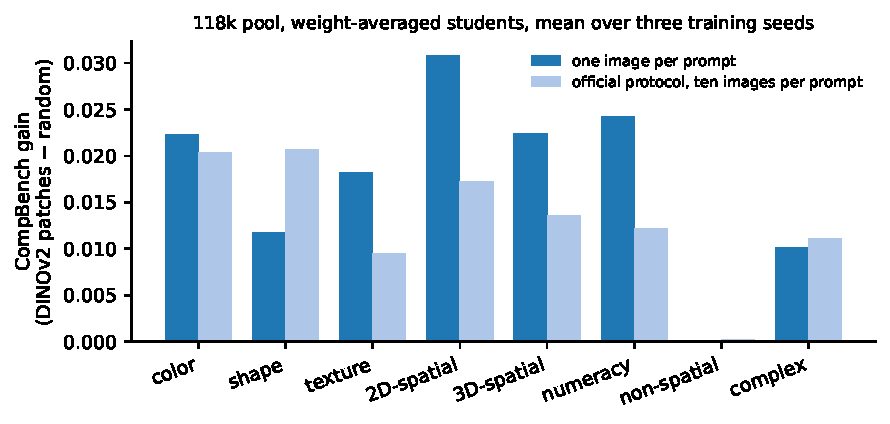
\includegraphics[width=\textwidth]{figs/per_category_gap.pdf}
\caption{Per-category CompBench gain of DINOv2 patch selection over random selection at 118k (three-seed means of the averaged students) under both protocols. The gain is spread over the attribute-binding, spatial and counting categories and is zero on non-spatial, whose CLIPScore evaluator does not separate any two students in this work.}
\label{fig:percat}
\end{minipage}\hfill
\begin{minipage}[t]{0.42\textwidth}
\centering
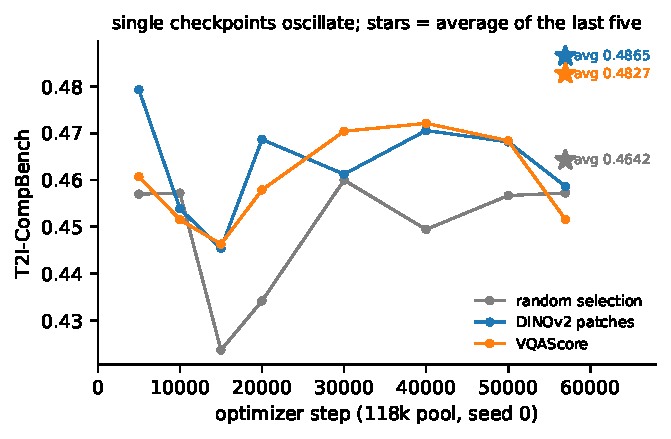
\includegraphics[width=\textwidth]{figs/checkpoint_curve.pdf}
\caption{CompBench of every saved checkpoint of the seed-0 118k runs; the star marks the weight average of the last five checkpoints of each arm (Section~\ref{sec:averaging}).}
\label{fig:curve}
\end{minipage}
\end{figure}

\subsection{Fidelity, three seeds}
Table~\ref{tab:fid118k} gives fidelity per seed. The 0.05 to 0.06 CMMD advantage of the scored student holds on every seed, far outside the $\pm0.01$ bootstrap interval, and so do precision and recall. FID is within its split-half spread.

\begin{table}[ht]
\centering
\caption{Fidelity at 118k, weight-averaged students, 5,000 COCO \texttt{val2017} captions, 4 steps, $w=1$, per training seed (s0 / s1 / s2).}
\label{tab:fid118k}
\resizebox{\textwidth}{!}{%
\begin{tabular}{l c c c c}
\toprule
Arm & FID $\downarrow$ & CMMD $\downarrow$ & Precision $\uparrow$ & Recall $\uparrow$ \\
\midrule
random (baseline) & 31.08 / 30.97 / 31.44 & 0.84 / 0.84 / 0.83 & 0.485 / 0.489 / 0.503 & 0.059 / 0.066 / 0.062 \\
DINOv2 patches & 30.98 / 30.83 / 31.47 & \textbf{0.78 / 0.79 / 0.78} & \textbf{0.522 / 0.511 / 0.522} & \textbf{0.071 / 0.068 / 0.063} \\
VQAScore (seed 0) & 30.45 & 0.79 & 0.510 & 0.061 \\
\midrule
Teacher, 28 steps, $w=7$ & 29.21 & 0.64 & 0.549 & 0.156 \\
\bottomrule
\end{tabular}}
\end{table}

\subsection{Why averaging is needed}
\label{sec:averaging}
Table~\ref{tab:curve} and Figure~\ref{fig:curve} evaluate every saved checkpoint of the three seed-0 runs. Consecutive checkpoints of one run differ by up to 0.035 CompBench, which is larger than the effect. The cause is the fixed-size normalised step (Section~\ref{sec:distill}) with no averaging: the weights move on a plateau and each checkpoint samples a different point of it. Paired across the eight checkpoints, the patch arm is ahead of random on CompBench by $+0.014$ on average (7 of 8 checkpoints, $p=0.02$) and the VQAScore arm by $+0.010$ (6 of 8, $p=0.05$). Averaging the last five checkpoints raised every arm and moved the scored arms most. Over the three seeds, the raw final checkpoints give a patch-minus-random gap of only $+0.007$ ($+0.001$, $+0.003$, $+0.017$; $p=0.003$) against $+0.0175$ for the averaged weights, so averaging is not optional at this scale, and it is applied identically to every arm.

\begin{table}[ht]
\centering
\caption{CompBench of every saved checkpoint of the seed-0 118k runs. The last row is the weight average of the last five checkpoints.}
\label{tab:curve}
\resizebox{\textwidth}{!}{%
\begin{tabular}{r r c c c c c}
\toprule
Step & Caption visits & random & DINOv2 patches & VQAScore & patch $\Delta$ & VQAScore $\Delta$ \\
\midrule
5,000 & 20,000 & 0.4570 & 0.4793 & 0.4607 & $+0.0223$ & $+0.0037$ \\
10,000 & 40,000 & 0.4572 & 0.4539 & 0.4515 & $-0.0033$ & $-0.0057$ \\
15,000 & 60,000 & 0.4237 & 0.4454 & 0.4463 & $+0.0217$ & $+0.0226$ \\
20,000 & 80,000 & 0.4342 & 0.4687 & 0.4579 & $+0.0345$ & $+0.0237$ \\
30,000 & 120,000 & 0.4600 & 0.4612 & 0.4704 & $+0.0013$ & $+0.0104$ \\
40,000 & 160,000 & 0.4494 & 0.4706 & 0.4721 & $+0.0211$ & $+0.0227$ \\
50,000 & 200,000 & 0.4567 & 0.4682 & 0.4684 & $+0.0115$ & $+0.0117$ \\
56,974 & 227,896 & 0.4573 & 0.4587 & 0.4516 & $+0.0014$ & $-0.0056$ \\
\midrule
average of last 5 & & 0.4642 & 0.4865 & 0.4827 & $+0.0222$ & $+0.0185$ \\
\bottomrule
\end{tabular}}
\end{table}


The averaging also improved fidelity for every arm at seed 0: CMMD went from 0.87 to 0.84 for random, 0.86 to 0.78 for the patch arm and 0.87 to 0.79 for the VQAScore arm.

\subsection{Optimizer batch size}
\label{sec:batch}
Every update above processes four captions, one per GPU. To test whether the oscillation or the gap depends on that, both arms were retrained at seed 0 with gradient accumulation over four captions per GPU: 16 captions per update, 14,244 updates for the same two passes over the data, checkpoints every 1,250 updates so that the last-five average spans the same data window. Nothing else changed. Table~\ref{tab:batch} gives the result. The selection gap is unchanged ($+0.0221$ against $+0.0223$ for this seed at batch 4). Batch 16 lifts both arms by the same $+0.005$, which is not significant at one seed. It removes the oscillation of the random arm (raw final and average within 0.001) but not of the scored arm (0.012 apart), so averaging remains necessary, and batch 4 with averaging remains the reported configuration. This row is a robustness check.

\begin{table}[ht]
\centering
\caption{Optimizer batch size at 118k, seed 0. Batch 16 uses gradient accumulation over four captions per GPU at the same data budget. CompBench / GenEval2$\times100$.}
\label{tab:batch}
\resizebox{\textwidth}{!}{%
\begin{tabular}{l c c c c}
\toprule
Batch (updates) & random, raw final & random, averaged & DINOv2 patches, raw final & DINOv2 patches, averaged \\
\midrule
4 (56,974) & 0.4573 / 19.51 & 0.4642 / 20.61 & 0.4587 / 20.18 & 0.4865 / 22.05 \\
16 (14,244) & 0.4684 / 20.28 & 0.4695 / 21.22 & 0.4796 / 20.90 & \textbf{0.4916 / 22.68} \\
\midrule
gap at batch 16, averaged & \multicolumn{4}{c}{$+0.0221$ CompBench ($p=4\times10^{-10}$), $+1.45$ GenEval2 ($p=0.10$)} \\
\bottomrule
\end{tabular}}
\end{table}

\subsection{Number of candidates}
\label{sec:n8}
The cache was extended from four to eight candidates per caption with the same seed convention (candidate $j$ from seed $1000\cdot\texttt{idx}+j$, $j=4,\dots,7$), keeping the random arm's stored draw, so the $N=4$ arms remain the exact control. Offline, best-of-eight raises the VQAScore oracle on this pool from 0.9335 to 0.9487 (headroom over the random pick $+0.094\to+0.109$, 16\% more), and the DINOv2-selected candidate from 0.8796 to 0.8862, the same 43\% of the respective headroom. Trained with argmax over eight candidates, three seeds, the averaged students score 0.4862 / 0.4859 / 0.4838 CompBench (mean 0.4853) and 21.68 / 21.44 / 21.50 GenEval2 (21.54): $+0.0010$ ($p=0.64$) and $-0.04$ against the $N=4$ arm, a null. Both arms are about $+0.018$ over random. Four candidates saturate this scorer on this teacher; the extra offline headroom of eight does not convert into a trained gain.

\clearpage
\section{Selection rule: argmax, Boltzmann weighting and sampling}
\label{sec:selrule}

Argmax selection is one point on a family of rules; Table~\ref{tab:arms} defines every arm of this section against the objective of Equation~\ref{eq:unified}, and Figures~\ref{fig:allarms} to~\ref{fig:heatmap} compare them all at once. The natural alternative to argmax weights the candidates by a Boltzmann distribution over the raw scores,
\begin{equation}
\pi_j=\frac{\exp(S_j/T)}{\sum_{l=1}^{4}\exp(S_l/T)},
\end{equation}
which recovers argmax as $T\to0$ and uniform weighting as $T\to\infty$. Two estimators of the weighted objective $\sum_j\pi_j\mathcal{L}_j$ were trained. \emph{Exact} weighting rolls out all four candidates and back-propagates each candidate's loss with weight $\pi_j$: four teacher rollouts and four student passes per caption, 2.3 times the wall-clock of the single-candidate trainer (3.5 h against 1.2 h per 3k run on one H200), at the same peak memory because candidates are back-propagated one at a time. \emph{Sampled} weighting draws one candidate $J\sim\pi$ on every visit of the caption and trains on it alone at single-candidate cost. Every candidate is evaluated at its own trajectory, so neither estimator regresses onto an averaged target; the two have the same expected gradient, $\mathbb{E}[g_J]=\sum_j\pi_jg_j=g_F$, but not the same optimizer update (Section~\ref{sec:graddiag}). Three controls complete the design: the random baseline, which draws one candidate per caption uniformly and keeps it; a \emph{uniform-visit} arm that redraws uniformly on every visit; and a \emph{frozen} Boltzmann arm that draws $J_c\sim\pi_c$ once per caption and keeps it, which has the sampled arm's selection distribution without per-visit resampling. A same-caption Monte-Carlo estimator ($M$ independent draws per visit, losses weighted by their counts, one clipped step) is implemented in the release code and was not run.

\subsection{Selection entropy and effective sample size}
The temperature is calibrated on the scores themselves. Figure~\ref{fig:entropy} and Table~\ref{tab:scorestats} summarise the DINOv2 patch score over the four candidates of a caption. Within a caption the scores have a standard deviation of 0.070 (range 0.18, margin between the best and the second-best candidate 0.05); between captions the mean score varies twice as much (0.14), which is why scores are only ever compared within a caption. Two effective-count summaries of the weights are used and they are not interchangeable: the entropy count $N_H=\exp H(\pi)$ and the Kish count $N_K=1/\sum_j\pi_j^2$. At $T=0.04$ the median $N_H$ is 2.5 and the median $N_K$ is 2.2, with a mean argmax weight of 0.63; at $T=0.08$ they are 3.3 and 3.0. The Kish count is the one tied to resampling: the probability that two independent visits train on different candidates is $1-\sum_j\pi_j^2=1-1/N_K$, 0.49 at $T=0.04$ and 0.63 at $T=0.08$, and in the two visits per caption of the 3k configuration the sampled arm sees on average 1.48 (1.63) distinct candidates of the four that the exact arm sees on every visit. The 3k and 118k pools have the same statistics, so a temperature calibrated on one transfers to the other. Stronger teachers compress the candidates: on the 16-step $w=4.5$ and 28-step caches the within-caption spread almost halves (0.041 and 0.038) and the entropy at a fixed temperature rises (0.75 and 0.76 at $T=0.04$). This is the offline face of the vanishing selection gain of Section~\ref{sec:k28}.

\begin{table}[ht]
\centering
\caption{DINOv2 patch score statistics per candidate cache ($N=4$): within-caption standard deviation, mean range, mean margin between the two best candidates, and the mean normalised entropy and median entropy count $N_H$ of the Boltzmann weights at the two temperatures used in training. On the 3k cache the median Kish count $N_K$ is 2.2 at $T=0.04$ and 3.0 at $T=0.08$.}
\label{tab:scorestats}
\resizebox{\textwidth}{!}{%
\begin{tabular}{l r c c c cc cc}
\toprule
 & & & & & \multicolumn{2}{c}{$T=0.04$} & \multicolumn{2}{c}{$T=0.08$} \\
Cache (teacher) & captions & within std & range & top-2 margin & entropy & $N_H$ & entropy & $N_H$ \\
\midrule
3k, 8 steps, $w=7$ & 3,000 & 0.069 & 0.175 & 0.049 & 0.63 & 2.54 & 0.82 & 3.33 \\
118k, 8 steps, $w=7$ & 113,948 & 0.070 & 0.179 & 0.051 & 0.62 & 2.52 & 0.81 & 3.32 \\
3k, 16 steps, $w=4.5$ & 3,000 & 0.041 & 0.105 & 0.034 & 0.75 & 3.01 & 0.91 & 3.65 \\
3k, 28 steps, $w=7$ & 3,000 & 0.038 & 0.099 & 0.033 & 0.76 & 3.09 & 0.91 & 3.68 \\
\bottomrule
\end{tabular}}
\end{table}

\begin{figure}[ht]
\centering
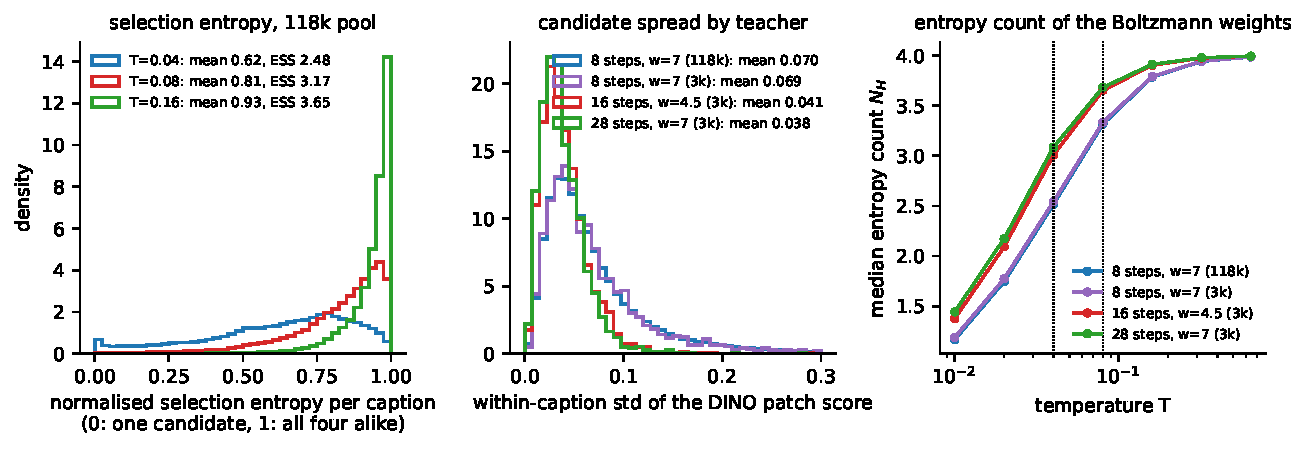
\includegraphics[width=\textwidth]{figs/score_entropy.pdf}
\caption{Left: distribution over captions of the normalised selection entropy at three temperatures (118k pool). Middle: within-caption spread of the DINOv2 patch score for the four caches; stronger teachers leave less to select on. Right: median entropy count $N_H$ of the Boltzmann weights as a function of temperature; the two temperatures used in training are marked.}
\label{fig:entropy}
\end{figure}

\subsection{Protocol and statistics}
\label{sec:selstats}
All arms were trained on the 3k pool with the 3k configuration, three seeds each, from one frozen copy of the trainer; the random and argmax arms were retrained alongside the new ones so that every contrast is a one-factor change. Their absolute level is 0.008 below the earlier runs of Table~\ref{tab:main3k} (a different launch, within the seed spread), so contrasts are read within this section. Every arm is evaluated under two protocols: the raw final checkpoint, and the uniform average of the checkpoints saved at 2,000, 4,000 and 6,000 updates, applied with the same rule to every arm. The averaging is the 3k analogue of the last-five average that the 118k results require (Section~\ref{sec:averaging}); it raises every arm by 0.014 to 0.027 CompBench, and it matters for the comparison below because arms differ in how much their final iterate wanders.

Uncertainty is reported at the level of training runs. For a contrast between arms A and B the three seed-paired differences (seed $s$ of A minus seed $s$ of B; at equal seed the arms share the caption order and the $\Delta$ draws) give a mean, a standard deviation, a 95\% $t$-interval and a one-sample $t$-test with two degrees of freedom. Three seeds resolve a difference of about 0.01 CompBench and nothing on GenEval2, whose seed spread is 1 to 2 points. The prompt-level $p$-values of the paired tests used elsewhere in this document describe uncertainty over prompts for the seed-mean model, not over repeated training, and are not used to compare selection rules. A non-significant contrast is reported as ``no detected improvement''; none of the tests here is an equivalence test.

\subsection{Result}
Tables~\ref{tab:selrule} to~\ref{tab:selcontrasts_avg} and Figure~\ref{fig:selrule} give the result.

\begin{table}[ht]
\centering
\caption{Selection rule, 3k pool, three seeds. CompBench per seed (s0 / s1 / s2) and mean $\pm$ standard deviation over seeds, for the raw final checkpoint and for the uniform average of the checkpoints at 2k, 4k and 6k updates; GenEval2$\times100$ seed means under both protocols; GPU-hours per training run on one H200. \emph{exact}: every candidate's loss weighted by $\pi_j$; \emph{sampled}: one draw from $\pi$ per visit; \emph{kept}: one draw from $\pi$ per caption, fixed for the run.}
\label{tab:selrule}
\resizebox{\textwidth}{!}{%
\begin{tabular}{l cc cc cc c}
\toprule
 & \multicolumn{2}{c}{CompBench, raw final} & \multicolumn{2}{c}{CompBench, averaged} & \multicolumn{2}{c}{GenEval2} & \\
Rule & s0 / s1 / s2 & mean $\pm$ sd & s0 / s1 / s2 & mean $\pm$ sd & raw & avg. & GPU-h \\
\midrule
random (fixed draw) & 0.4491 / 0.4393 / 0.4612 & 0.4499 $\pm$ 0.0110 & 0.4756 / 0.4724 / 0.4732 & 0.4738 $\pm$ 0.0017 & 21.12 & 22.53 & 1.2 \\
argmax & 0.4690 / 0.4591 / 0.4825 & \textbf{0.4702 $\pm$ 0.0118} & 0.4849 / 0.4861 / 0.4909 & \textbf{0.4873 $\pm$ 0.0032} & 22.46 & 23.73 & 1.2 \\
\midrule
Boltzmann $T{=}0.04$, exact & 0.4714 / 0.4709 / 0.4684 & 0.4703 $\pm$ 0.0016 & 0.4855 / 0.4859 / 0.4805 & 0.4840 $\pm$ 0.0030 & 22.65 & 23.66 & 3.5 \\
Boltzmann $T{=}0.08$, exact & 0.4687 / 0.4688 / 0.4693 & 0.4689 $\pm$ 0.0003 & 0.4751 / 0.4862 / 0.4686 & 0.4766 $\pm$ 0.0089 & 22.17 & 23.45 & 3.6 \\
uniform ($T\to\infty$), exact & 0.4586 / 0.4536 / 0.4550 & 0.4557 $\pm$ 0.0025 & 0.4710 / 0.4803 / 0.4710 & 0.4741 $\pm$ 0.0054 & 21.28 & 23.50 & 3.6 \\
\midrule
Boltzmann $T{=}0.04$, sampled & 0.4489 / 0.4451 / 0.4745 & 0.4562 $\pm$ 0.0160 & 0.4820 / 0.4795 / 0.4878 & 0.4831 $\pm$ 0.0043 & 21.18 & 23.87 & 1.2 \\
Boltzmann $T{=}0.08$, sampled & 0.4459 / 0.4389 / 0.4704 & 0.4517 $\pm$ 0.0165 & 0.4785 / 0.4824 / 0.4810 & 0.4806 $\pm$ 0.0020 & 22.37 & 23.50 & 1.2 \\
uniform-visit (redraw per visit) & 0.4520 / 0.4290 / 0.4456 & 0.4422 $\pm$ 0.0118 & 0.4744 / 0.4723 / 0.4780 & 0.4749 $\pm$ 0.0029 & 20.59 & 22.16 & 1.2 \\
\midrule
Boltzmann $T{=}0.04$, one draw per caption, kept & 0.4699 / 0.4405 / 0.4804 & 0.4636 $\pm$ 0.0207 & 0.4842 / 0.4840 / 0.4894 & 0.4858 $\pm$ 0.0030 & 21.77 & 24.17 & 1.2 \\
\bottomrule
\end{tabular}}
\end{table}


\begin{table}[ht]
\centering
\caption{Seed-paired CompBench contrasts between selection rules, raw final checkpoints (seed $s$ of the first arm minus seed $s$ of the second; the arms share caption order and $\Delta$ draws at equal seed): per-seed differences, mean $\pm$ standard deviation over seeds, 95\% $t$-interval and the seed-level $t$-test with $n=3$.}
\label{tab:selcontrasts}
\resizebox{\textwidth}{!}{%
\begin{tabular}{l c c}
\toprule
Contrast & per seed & mean $\pm$ sd [95\% CI] ($p$) \\
\midrule
\multicolumn{3}{l}{\emph{against the random baseline}} \\
argmax vs random (fixed draw) & +0.0199 / +0.0198 / +0.0213 & $+0.0203 \pm 0.0008$ [$+0.018$, $+0.022$] ($p=0.001$) \\
Boltzmann $T{=}0.04$, exact vs random (fixed draw) & +0.0223 / +0.0317 / +0.0072 & $+0.0204 \pm 0.0124$ [$-0.010$, $+0.051$] ($p=0.10$) \\
Boltzmann $T{=}0.08$, exact vs random (fixed draw) & +0.0195 / +0.0295 / +0.0080 & $+0.0190 \pm 0.0107$ [$-0.008$, $+0.046$] ($p=0.09$) \\
uniform ($T\to\infty$), exact vs random (fixed draw) & +0.0094 / +0.0144 / -0.0063 & $+0.0058 \pm 0.0108$ [$-0.021$, $+0.033$] ($p=0.45$) \\
Boltzmann $T{=}0.04$, sampled vs random (fixed draw) & -0.0002 / +0.0059 / +0.0132 & $+0.0063 \pm 0.0067$ [$-0.010$, $+0.023$] ($p=0.25$) \\
Boltzmann $T{=}0.08$, sampled vs random (fixed draw) & -0.0032 / -0.0003 / +0.0092 & $+0.0019 \pm 0.0065$ [$-0.014$, $+0.018$] ($p=0.67$) \\
uniform-visit (redraw per visit) vs random (fixed draw) & +0.0028 / -0.0102 / -0.0157 & $-0.0077 \pm 0.0095$ [$-0.031$, $+0.016$] ($p=0.30$) \\
Boltzmann $T{=}0.04$, one draw per caption, kept vs random (fixed draw) & +0.0208 / +0.0013 / +0.0192 & $+0.0138 \pm 0.0109$ [$-0.013$, $+0.041$] ($p=0.16$) \\
\midrule
\multicolumn{3}{l}{\emph{against argmax}} \\
Boltzmann $T{=}0.04$, exact vs argmax & +0.0024 / +0.0119 / -0.0141 & $+0.0001 \pm 0.0131$ [$-0.033$, $+0.033$] ($p=1.00$) \\
Boltzmann $T{=}0.08$, exact vs argmax & -0.0004 / +0.0097 / -0.0132 & $-0.0013 \pm 0.0115$ [$-0.030$, $+0.027$] ($p=0.86$) \\
uniform ($T\to\infty$), exact vs argmax & -0.0105 / -0.0054 / -0.0276 & $-0.0145 \pm 0.0116$ [$-0.043$, $+0.014$] ($p=0.16$) \\
Boltzmann $T{=}0.04$, sampled vs argmax & -0.0201 / -0.0140 / -0.0080 & $-0.0140 \pm 0.0060$ [$-0.029$, $+0.001$] ($p=0.06$) \\
Boltzmann $T{=}0.04$, one draw per caption, kept vs argmax & +0.0009 / -0.0186 / -0.0021 & $-0.0066 \pm 0.0105$ [$-0.033$, $+0.019$] ($p=0.39$) \\
\midrule
\multicolumn{3}{l}{\emph{estimator and persistence}} \\
Boltzmann $T{=}0.04$, exact vs Boltzmann $T{=}0.04$, sampled & +0.0225 / +0.0258 / -0.0061 & $+0.0141 \pm 0.0175$ [$-0.029$, $+0.058$] ($p=0.30$) \\
Boltzmann $T{=}0.04$, one draw per caption, kept vs Boltzmann $T{=}0.04$, sampled & +0.0210 / -0.0046 / +0.0060 & $+0.0075 \pm 0.0129$ [$-0.025$, $+0.039$] ($p=0.42$) \\
uniform ($T\to\infty$), exact vs uniform-visit (redraw per visit) & +0.0066 / +0.0246 / +0.0094 & $+0.0135 \pm 0.0097$ [$-0.011$, $+0.038$] ($p=0.14$) \\
\bottomrule
\end{tabular}}
\end{table}

\begin{table}[ht]
\centering
\caption{Seed-paired CompBench contrasts between selection rules, averaged checkpoints (2k, 4k and 6k updates) (seed $s$ of the first arm minus seed $s$ of the second; the arms share caption order and $\Delta$ draws at equal seed): per-seed differences, mean $\pm$ standard deviation over seeds, 95\% $t$-interval and the seed-level $t$-test with $n=3$.}
\label{tab:selcontrasts_avg}
\resizebox{\textwidth}{!}{%
\begin{tabular}{l c c}
\toprule
Contrast & per seed & mean $\pm$ sd [95\% CI] ($p$) \\
\midrule
\multicolumn{3}{l}{\emph{against the random baseline}} \\
argmax vs random (fixed draw) & +0.0092 / +0.0137 / +0.0177 & $+0.0135 \pm 0.0042$ [$+0.003$, $+0.024$] ($p=0.03$)  \\
Boltzmann $T{=}0.04$, exact vs random (fixed draw) & +0.0099 / +0.0135 / +0.0073 & $+0.0102 \pm 0.0031$ [$+0.002$, $+0.018$] ($p=0.03$)  \\
Boltzmann $T{=}0.08$, exact vs random (fixed draw) & -0.0006 / +0.0138 / -0.0046 & $+0.0029 \pm 0.0097$ [$-0.021$, $+0.027$] ($p=0.66$)  \\
uniform ($T\to\infty$), exact vs random (fixed draw) & -0.0046 / +0.0079 / -0.0022 & $+0.0004 \pm 0.0067$ [$-0.016$, $+0.017$] ($p=0.93$)  \\
Boltzmann $T{=}0.04$, sampled vs random (fixed draw) & +0.0063 / +0.0071 / +0.0146 & $+0.0093 \pm 0.0046$ [$-0.002$, $+0.021$] ($p=0.07$)  \\
Boltzmann $T{=}0.08$, sampled vs random (fixed draw) & +0.0029 / +0.0100 / +0.0077 & $+0.0069 \pm 0.0036$ [$-0.002$, $+0.016$] ($p=0.08$)  \\
uniform-visit (redraw per visit) vs random (fixed draw) & -0.0013 / -0.0001 / +0.0048 & $+0.0012 \pm 0.0032$ [$-0.007$, $+0.009$] ($p=0.60$)  \\
Boltzmann $T{=}0.04$, one draw per caption, kept vs random (fixed draw) & +0.0085 / +0.0116 / +0.0162 & $+0.0121 \pm 0.0038$ [$+0.003$, $+0.022$] ($p=0.03$)  \\
\midrule
\multicolumn{3}{l}{\emph{against argmax}} \\
Boltzmann $T{=}0.04$, exact vs argmax & +0.0006 / -0.0001 / -0.0104 & $-0.0033 \pm 0.0062$ [$-0.019$, $+0.012$] ($p=0.45$)  \\
Boltzmann $T{=}0.08$, exact vs argmax & -0.0098 / +0.0001 / -0.0223 & $-0.0107 \pm 0.0112$ [$-0.039$, $+0.017$] ($p=0.24$)  \\
uniform ($T\to\infty$), exact vs argmax & -0.0139 / -0.0058 / -0.0199 & $-0.0132 \pm 0.0071$ [$-0.031$, $+0.004$] ($p=0.08$)  \\
Boltzmann $T{=}0.04$, sampled vs argmax & -0.0029 / -0.0066 / -0.0031 & $-0.0042 \pm 0.0021$ [$-0.009$, $+0.001$] ($p=0.07$)  \\
Boltzmann $T{=}0.04$, one draw per caption, kept vs argmax & -0.0007 / -0.0021 / -0.0016 & $-0.0015 \pm 0.0007$ [$-0.003$, $+0.000$] ($p=0.07$)  \\
\midrule
\multicolumn{3}{l}{\emph{estimator and persistence}} \\
Boltzmann $T{=}0.04$, exact vs Boltzmann $T{=}0.04$, sampled & +0.0036 / +0.0065 / -0.0073 & $+0.0009 \pm 0.0073$ [$-0.017$, $+0.019$] ($p=0.85$)  \\
Boltzmann $T{=}0.04$, one draw per caption, kept vs Boltzmann $T{=}0.04$, sampled & +0.0022 / +0.0045 / +0.0015 & $+0.0028 \pm 0.0016$ [$-0.001$, $+0.007$] ($p=0.09$)  \\
uniform ($T\to\infty$), exact vs uniform-visit (redraw per visit) & -0.0033 / +0.0080 / -0.0070 & $-0.0008 \pm 0.0078$ [$-0.020$, $+0.019$] ($p=0.88$)  \\
\bottomrule
\end{tabular}}
\end{table}

\begin{table}[ht]
\centering
\caption{Fidelity of the $T{=}0.04$ selection-rule arms and the latent-scorer arms on 5,000 COCO \texttt{val2017} captions, 4 steps, $w=1$: per seed (s0 / s1 / s2) and seed mean in brackets, for the raw final checkpoints and for the averaged checkpoints. CMMD bootstrap intervals are $\pm0.01$ per model; FID differences below its split-half spread of about 0.5 should not be read.}
\label{tab:selfid}
\resizebox{\textwidth}{!}{%
\begin{tabular}{l l c c c c}
\toprule
Rule & checkpoint & FID $\downarrow$ & CMMD $\downarrow$ & Precision $\uparrow$ & Recall $\uparrow$ \\
\midrule
random (fixed draw) & raw final & 32.91 / 33.16 / 31.17 (32.41) & 0.91 / 0.96 / 0.97 (0.95) & 0.456 / 0.436 / 0.414 (0.435) & 0.045 / 0.046 / 0.037 (0.043) \\
argmax & raw final & 31.90 / 30.57 / 29.62 (30.70) & 0.89 / 0.94 / 0.83 (0.89) & 0.455 / 0.450 / 0.485 (0.463) & 0.052 / 0.047 / 0.060 (0.053) \\
Boltzmann $T{=}0.04$, exact & raw final & 30.97 / 29.43 / 31.22 (30.54) & 0.85 / 0.87 / 0.85 (0.86) & 0.488 / 0.461 / 0.504 (0.484) & 0.058 / 0.051 / 0.050 (0.053) \\
Boltzmann $T{=}0.04$, sampled & raw final & 32.90 / 32.01 / 31.40 (32.10) & 0.90 / 1.02 / 0.93 (0.95) & 0.464 / 0.434 / 0.449 (0.449) & 0.040 / 0.040 / 0.043 (0.041) \\
Boltzmann $T{=}0.04$, one draw per caption, kept & raw final & 32.64 / 33.32 / 32.37 (32.78) & 0.89 / 0.98 / 0.90 (0.92) & 0.445 / 0.444 / 0.443 (0.444) & 0.052 / 0.039 / 0.047 (0.046) \\
latent scorer, argmax & raw final & 33.09 / 31.08 / 31.66 (31.94) & 0.85 / 0.90 / 0.91 (0.89) & 0.507 / 0.429 / 0.449 (0.462) & 0.053 / 0.048 / 0.042 (0.048) \\
latent scorer, Boltzmann $T{=}0.04$, exact & raw final & 31.79 / 31.60 / 31.23 (31.54) & 0.81 / 0.83 / 0.85 (0.83) & 0.512 / 0.492 / 0.497 (0.500) & 0.056 / 0.057 / 0.053 (0.055) \\
\midrule
random (fixed draw) & averaged & 30.58 / 30.45 / 30.24 (30.42) & 0.79 / 0.85 / 0.87 (0.84) & 0.507 / 0.474 / 0.457 (0.479) & 0.056 / 0.055 / 0.051 (0.054) \\
argmax & averaged & 30.53 / 29.85 / 29.99 (30.12) & 0.83 / 0.80 / 0.77 (0.80) & 0.489 / 0.495 / 0.484 (0.489) & 0.062 / 0.067 / 0.070 (0.066) \\
Boltzmann $T{=}0.04$, exact & averaged & 30.37 / 29.81 / 30.75 (30.31) & 0.79 / 0.80 / 0.79 (0.79) & 0.508 / 0.489 / 0.507 (0.501) & 0.066 / 0.069 / 0.059 (0.065) \\
Boltzmann $T{=}0.04$, sampled & averaged & 29.83 / 30.21 / 30.86 (30.30) & 0.81 / 0.84 / 0.81 (0.82) & 0.484 / 0.457 / 0.486 (0.476) & 0.062 / 0.059 / 0.062 (0.061) \\
Boltzmann $T{=}0.04$, one draw per caption, kept & averaged & 30.98 / 31.11 / 31.05 (31.05) & 0.84 / 0.81 / 0.84 (0.83) & 0.478 / 0.484 / 0.474 (0.479) & 0.062 / 0.066 / 0.061 (0.063) \\
latent scorer, argmax & averaged & 31.01 / 29.84 / 30.71 (30.52) & 0.82 / 0.80 / 0.82 (0.81) & 0.495 / 0.475 / 0.485 (0.485) & 0.061 / 0.062 / 0.057 (0.060) \\
latent scorer, Boltzmann $T{=}0.04$, exact & averaged & 30.23 / 30.68 / 30.47 (30.46) & 0.78 / 0.80 / 0.80 (0.79) & 0.512 / 0.493 / 0.509 (0.505) & 0.067 / 0.066 / 0.067 (0.067) \\
\bottomrule
\end{tabular}}
\end{table}


\begin{figure}[ht]
\centering
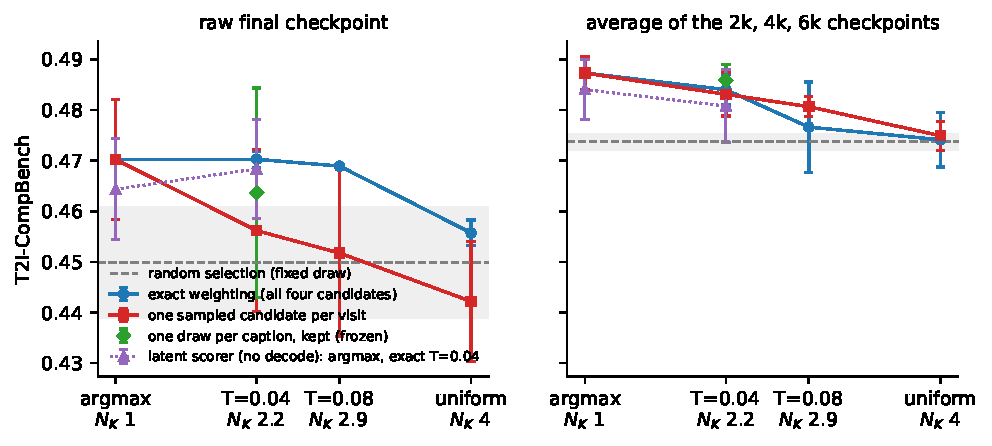
\includegraphics[width=\textwidth]{figs/selection_rule.pdf}
\caption{CompBench of the selection rules as a function of the Kish count of their weights, raw final checkpoints (left) and the average of the 2k, 4k and 6k checkpoints (right). Points are seed means, bars are seed standard deviations, the grey band is the random baseline. On raw checkpoints the sampled arms fall away from argmax while the exact arms stay flat; after identical averaging the two estimators coincide and the ordering follows the weight on the best candidate.}
\label{fig:selrule}
\end{figure}

\begin{itemize}
\item \textbf{Argmax over random is the one contrast established at the level of training runs:} $+0.0203\pm0.0008$ on raw checkpoints ($p=0.001$) and $+0.0135\pm0.0042$ after averaging ($p=0.03$).
\item \textbf{Exact Boltzmann weighting shows no detected improvement over argmax} at either temperature: $T=0.04$ is $+0.0001\pm0.013$ raw and $-0.003\pm0.006$ averaged; $T=0.08$ is $-0.001\pm0.012$ raw and $-0.011\pm0.011$ averaged. The averaged $T=0.04$ interval is $\pm0.015$, so a soft rule within 0.01 of argmax is not excluded; one that is better is not supported, and it costs 2.3 times the compute.
\item \textbf{Score-informed weighting is what matters.} At the same exact compute, $T=0.04$ is ahead of uniform weighting by $0.0145$ on raw checkpoints (positive on every seed) and by $+0.010$ (per seed $+0.015$, $+0.006$, $+0.010$) after averaging, and uniform weighting of all four candidates is within noise of the random baseline under both protocols. Exposure to more trajectories per caption is worth little on its own.
\item \textbf{The sampled estimator's deficit is mostly a property of its final iterate.} On raw checkpoints the sampled $T=0.04$ arm is $0.014\pm0.006$ below argmax and $0.014\pm0.018$ below exact weighting; after averaging the gaps are $0.004\pm0.002$ and $-0.001\pm0.007$. The sampled arm's raw checkpoints vary four times more across seeds than its averaged weights (0.016 against 0.004). What remains after averaging is of the size the optimizer-level differences of Section~\ref{sec:graddiag} can produce and is not resolved at three seeds.
\item \textbf{Persistence of the selected candidate is not established as a separate effect.} Redrawing uniformly on every visit is $0.008\pm0.010$ below the fixed random draw on raw checkpoints but $+0.001\pm0.003$ after averaging. The frozen Boltzmann arm, which keeps one draw from $\pi$ per caption, is $+0.008\pm0.013$ above the resampled arm on raw checkpoints and $+0.003\pm0.002$ after averaging (positive on all three seeds, $p=0.09$), and $0.0015\pm0.0007$ below argmax after averaging. Its raw checkpoints vary the most of all arms across seeds (0.021), since each seed also carries its own selection map; averaging removes that as well. Switching candidates changes the input trajectory and its target together, and in the two visits per caption of this configuration the sampled arm sees 1.5 distinct candidates on average, so target churn, candidate coverage and optimization variance are not separated by these controls.
\item \textbf{Stability.} On raw checkpoints the exact arms vary far less across seeds than the single-candidate arms (standard deviation 0.0016 and 0.0003 against 0.011 to 0.017); after averaging the difference is gone (0.003 and 0.009 against 0.002 to 0.004). Averaging four trajectories per update stabilises the iterate, not the solution.
\item \textbf{Fidelity.} Table~\ref{tab:selfid} gives FID, CMMD, precision and recall for the $T{=}0.04$ arms. On raw final checkpoints the exact arm has the best fidelity (CMMD 0.86 against 0.89 for argmax and 0.95 for both random and the resampled arm) and the resampled arm sits at the random level; after averaging every arm improves by about 0.1 CMMD and the differences shrink to within the seed spread (exact minus argmax $-0.007\pm0.031$, resampled minus argmax $+0.020\pm0.035$, frozen minus argmax $+0.030\pm0.035$). The one fidelity contrast that keeps its sign on every seed after averaging is exact against resampled, $-0.027\pm0.012$ CMMD and $+0.026$ precision ($p=0.06$): weighting all four candidates gives a slightly better distribution match than sampling one, with no alignment difference.
\item \textbf{GenEval2} does not separate any two selection rules at three seeds.
\end{itemize}

\subsection{Gradient diagnostic}
\label{sec:graddiag}
Equal expected gradients do not give equal optimizer updates. The trainer clips the global gradient norm to $\gamma=1$ and then applies AdamW, and clipping does not commute with expectation: $\mathbb{E}[C(g_J)]\neq C(\mathbb{E}[g_J])$ for $C(g)=g\min(1,\gamma/\lVert g\rVert)$, while Adam's second moment sees $\mathbb{E}[g_J\odot g_J]=g_F\odot g_F+\mathrm{Var}(g_J)$. To measure how large these effects are for this loss, all four candidate gradients of a caption were computed at two frozen model states, the pretrained initialisation and the argmax student of seed 0, on 48 held-out captions of the 118k pool (none in the 3k pool), with one $\Delta$ draw shared by the four candidates. Everything below is a function of the $4\times4$ Gram matrix of the candidate gradients and $\pi$ at $T=0.04$:
\begin{equation}
V_c=\sum_j\pi_j\lVert g_j-g_F\rVert^2,\qquad
B_c=\Big\lVert\sum_j\pi_jC(g_j)-C(g_F)\Big\rVert .
\end{equation}
Two references are computed per caption: the argmax candidate's gradient under a second $\Delta$ draw on the same trajectory, which is the gradient noise every arm carries, and the argmax candidate rolled out alone instead of in the four-candidate batch, which checks that batch shape is not a confound.

\begin{table}[ht]
\centering
\caption{Gradient diagnostic at $T=0.04$, 48 held-out captions, means over captions (medians in brackets). Every gradient is clipped: norms are 300 to 650 against $\gamma=1$. $g_F$ is the exact weighted gradient, $g_J$ the one-sample gradient, $C$ the clip.}
\label{tab:graddiag}
\resizebox{\textwidth}{!}{%
\begin{tabular}{l c c}
\toprule
 & argmax student (seed 0) & pretrained init \\
\midrule
mean pairwise cosine of the four candidate gradients & 0.17 [0.14] & 0.43 [0.43] \\
$\cos(g_{j^\star},g_F)$, argmax candidate against the exact gradient & 0.87 [0.92] & 0.91 [0.94] \\
candidate-sampling variance $V_c/\lVert g_F\rVert^2$ & 0.99 [0.76] & 0.51 [0.42] \\
Adam second-moment ratio $\sum_j\pi_j\lVert g_j\rVert^2/\lVert g_F\rVert^2$ & 1.99 [1.76] & 1.51 [1.42] \\
clipping difference $B_c/\lVert C(g_F)\rVert$ & 0.27 [0.27] & 0.17 [0.15] \\
$\cos\big(\mathbb{E}[C(g_J)],\,C(g_F)\big)$ & 0.990 [0.997] & 0.995 [0.998] \\
$\lVert\mathbb{E}[C(g_J)]\rVert/\lVert C(g_F)\rVert$ & 0.75 [0.75] & 0.85 [0.86] \\
\midrule
same candidate, second $\Delta$ draw: $\lVert g-g'\rVert^2/\lVert g\rVert^2$ & 0.78 [0.70] & 1.05 [0.59] \\
same candidate, second $\Delta$ draw: $\cos(g,g')$ & 0.67 & 0.65 \\
batched against single rollout: max state difference, $\cos$ of gradients & 0, 0.99999 & 0, 0.99999 \\
\bottomrule
\end{tabular}}
\end{table}

Three things follow. The candidate gradients of one caption are only weakly aligned (mean pairwise cosine 0.17 at the trained state), so the one-sample estimator carries a relative variance of order one: its noise power equals the signal power, and Adam's second moment is doubled. Under clipping its expected update is nearly parallel to the exact clipped update (cosine 0.99) but 25\% shorter, so the sampled arm takes systematically smaller steps in the same direction. And the $\Delta$ draw alone, which every arm resamples on every visit, produces gradient noise of the same order (relative squared difference 0.78 between two draws on the same trajectory), so candidate resampling roughly doubles a noise source that is already there rather than introducing a qualitatively new one. Batched and single rollouts give bit-identical states. The sampled estimator is therefore unbiased for the gradient of the weighted loss, and under clipping and AdamW it need not reproduce the exact estimator's optimisation; the measured differences are modest in direction and moderate in magnitude, which is consistent with the small residual gap after averaging and does not require contradictory targets to explain.

\subsection{A decode-free latent scorer}
\label{sec:latent}
The scorer of Section~\ref{sec:scorers} needs a VAE decode and a DINOv2 pass per candidate. Both are cheap offline (Section~\ref{sec:cost}), but a scorer that reads the terminal latent directly would remove them and could later be used inside a training loop. A latent scorer was therefore built and tested as a separate design decision from the selection rule. It replaces only the candidate side of the score: a projector $P$ maps the terminal latent $z_K$ to the DINOv2 patch-mean space, and the score is the cosine to the reference photograph's unchanged DINO embedding,
\begin{equation}
\hat S_j=\big\langle P(z_K^{(j)}),\,u^{\mathrm{pat}}(x^{\mathrm{ref}})\big\rangle .
\end{equation}
$P$ is a five-stage convolutional network with global pooling and a two-layer head (6.8M parameters). It was trained on 22,000 captions of the 118k pool, none of them in the 3k pool, with the terminal latents of their four cached candidates re-rolled from the cached seeds (the recomputed RGB scores match the cache to 0.002), on a cosine loss to the candidate's DINO embedding plus a within-caption ranking term, $\mathrm{KL}\big(\mathrm{softmax}(S/\tau)\,\|\,\mathrm{softmax}(\hat S/\tau)\big)$ at $\tau=0.04$, and validated on 2,000 further held-out captions. Training took five minutes on one GPU. The best epoch was chosen by selection regret on the validation captions, and the 3k pool's candidates were then scored once, offline, so the distillation arms below differ from the RGB arms only in the cache field they rank by.

\begin{table}[ht]
\centering
\caption{The latent scorer on the 3k pool, whose captions and photographs it never saw. Regret is the RGB DINO score of the RGB argmax minus that of the latent argmax; headroom is measured against the VQAScore best-of-four oracle as in Table~\ref{tab:headroom}.}
\label{tab:latent_offline}
\resizebox{\textwidth}{!}{%
\begin{tabular}{l c c}
\toprule
 & latent scorer & RGB DINOv2 patches \\
\midrule
top-1 agreement with the RGB argmax & 0.486 (chance 0.25) & 1 \\
within-caption Spearman with the RGB score & 0.47 & 1 \\
selection regret (RGB-score units; top-2 margin is 0.049) & 0.029 & 0 \\
VQAScore of the pick (random 0.843, oracle 0.933) & 0.874 & 0.882 \\
VQAScore headroom recovered & 34.0\% & 43.6\% \\
top-1 agreement with the VQAScore oracle & 0.32 & 0.36 \\
decode + scorer cost per caption & 0 & 61 + 32 ms \\
\bottomrule
\end{tabular}}
\end{table}

\begin{table}[ht]
\centering
\caption{Distillation with the latent scorer, 3k pool, three seeds, same configuration and trainer as Table~\ref{tab:selrule}. CompBench per seed and seed mean $\pm$ sd under both protocols; seed-paired contrasts after averaging.}
\label{tab:latent_arms}
\resizebox{\textwidth}{!}{%
\begin{tabular}{l cc cc c c}
\toprule
 & \multicolumn{2}{c}{raw final} & \multicolumn{2}{c}{averaged} & \multicolumn{2}{c}{averaged, seed-paired} \\
Rule & s0 / s1 / s2 & mean $\pm$ sd & s0 / s1 / s2 & mean $\pm$ sd & vs random & vs the RGB rule \\
\midrule
latent scorer, argmax & 0.4528 / 0.4701 / 0.4700 & 0.4643 $\pm$ 0.0100 & 0.4773 / 0.4877 / 0.4871 & 0.4840 $\pm$ 0.0059 & $+0.0103 \pm 0.0075$ & $-0.0033 \pm 0.0047$ \\
latent scorer, Boltzmann $T{=}0.04$, exact & 0.4732 / 0.4747 / 0.4572 & 0.4684 $\pm$ 0.0097 & 0.4818 / 0.4874 / 0.4731 & 0.4807 $\pm$ 0.0072 & $+0.0070 \pm 0.0076$ & $-0.0032 \pm 0.0045$ \\
RGB argmax (Table~\ref{tab:selrule}) & 0.4690 / 0.4591 / 0.4825 & 0.4702 $\pm$ 0.0118 & 0.4849 / 0.4861 / 0.4909 & 0.4873 $\pm$ 0.0032 & $+0.0135 \pm 0.0042$ & -- \\
RGB Boltzmann $T{=}0.04$, exact & 0.4714 / 0.4709 / 0.4684 & 0.4703 $\pm$ 0.0016 & 0.4855 / 0.4859 / 0.4805 & 0.4840 $\pm$ 0.0030 & $+0.0102 \pm 0.0031$ & -- \\
\bottomrule
\end{tabular}}
\end{table}

Table~\ref{tab:latent_arms} gives the distillation result. With the latent scorer, argmax selection is $+0.0103\pm0.0075$ CompBench over random after averaging and $0.0033\pm0.0047$ below RGB argmax; exact Boltzmann weighting is $+0.0070\pm0.0076$ over random and $0.0032\pm0.0045$ below its RGB counterpart, and as before it is not better than argmax. Neither latent arm is distinguishable from its RGB counterpart at three seeds, and the point estimates sit at about three quarters of the RGB gain, which is the fraction of the RGB scorer's offline headroom the projector recovers. Fidelity follows the same pattern (Table~\ref{tab:selfid}): after averaging, CMMD is 0.81 for latent argmax against 0.80 for RGB argmax and 0.79 for both exact arms, with seed-paired differences of $+0.013\pm0.032$ and $0.000\pm0.010$, and precision and recall within 0.006. One property of the projector matters for any use beyond offline selection: it was fitted to rank frozen-teacher candidates, and on the students' own 4-step samples its agreement with the RGB scorer drops (top-1 0.37, Spearman 0.22, against 0.51 and 0.46 on teacher candidates; the students' samples are also half as spread across seeds, 0.042 against 0.078), and fine-tuning it on 1,000 student latents does not restore it. It is a scorer of the teacher's candidate distribution. A scorer that reads the terminal latent therefore carries most of the selection signal at no decode cost, with a projector that trains in minutes; how much of the remaining quarter a larger projector, more training captions or a multi-scale readout would recover was not tested, and the same reference photograph is still required, since only the candidate side of the score moved into latent space.

\subsection{The projector as a reward inside training}
\label{sec:reward}
A scorer that reads latents can be applied inside the training loop, where decoding every prediction would not be affordable. This was tested as a reward term on the student's own predictions, with the projector both frozen and updated as the student changes. Before training, the precondition was measured: on the students' own 4-step samples the frozen projector agrees with the RGB scorer much less than on teacher candidates (Section~\ref{sec:latent}: top-1 0.37 against 0.51), and fine-tuning it offline on 1,000 student latents does not raise that, so the expectation on record was a small or null effect, to be judged by a hacking monitor rather than by the reward alone.

\paragraph{Design.}
At every update the reward $r=\langle P(\hat{x}_0),u^{\mathrm{pat}}(x^{\mathrm{ref}})\rangle$ is computed on the two clean estimates $\hat{x}_0$ from the least-noisy student inputs (the estimates from the noisier inputs are too blurry to score) and $-\lambda r$ is added to the consistency loss of the argmax arm, so the gradient flows through the frozen projector weights into the student. $\lambda$ was set from a probe of the two gradients on eight updates: at $\lambda=1$ the reward gradient has 0.25\% of the consistency gradient's norm (1.4 against 620), so $\lambda=80$ puts it at 20\%. Every 100 updates the 32 most recent predictions are decoded and scored with the RGB DINO scorer against their references, and the RGB score, the projector score and their correlation over the batch are logged; this is the monitor. In the \emph{refreshed} arm the projector then takes four AdamW steps on those decoded predictions (cosine to their DINO embeddings) mixed with replay of 2,000 teacher-candidate captions under the original loss, so it tracks the RGB scorer on the student's prediction distribution; in the \emph{frozen} arm it does not. Three seeds each, 3k configuration.

\begin{table}[ht]
\centering
\caption{Projector reward, 3k pool, three seeds. Left: the monitor at the start (updates 100 to 300) and the end (5,800 to 6,000) of training, means over seeds: DINO score of the decoded predictions under the projector (the reward) and under the RGB scorer, and their correlation over the 32 decoded latents. Right: CompBench and GenEval2 of the trained students, raw final and averaged checkpoints, with seed-paired contrasts against the argmax arm after averaging.}
\label{tab:reward}
\resizebox{\textwidth}{!}{%
\begin{tabular}{l cc cc cc c c c}
\toprule
 & \multicolumn{2}{c}{projector score} & \multicolumn{2}{c}{true RGB score} & \multicolumn{2}{c}{correlation} & CompBench & CompBench & vs argmax \\
Arm & start & end & start & end & start & end & raw & averaged & averaged \\
\midrule
argmax (reference, Table~\ref{tab:selrule}) & -- & -- & -- & -- & -- & -- & 0.4702 $\pm$ 0.0118 & 0.4873 $\pm$ 0.0032 & -- \\
argmax + reward, frozen projector & 0.396 & 0.427 & 0.589 & 0.579 & 0.32 & 0.36 & 0.4758 $\pm$ 0.0068 & 0.4847 $\pm$ 0.0075 & $-0.0026 \pm 0.0050$ \\
argmax + reward, refreshed projector & 0.398 & 0.435 & 0.589 & 0.578 & 0.33 & 0.41 & 0.4773 $\pm$ 0.0058 & 0.4876 $\pm$ 0.0096 & $+0.0003 \pm 0.0075$ \\
\bottomrule
\end{tabular}}
\end{table}

\begin{figure}[ht]
\centering
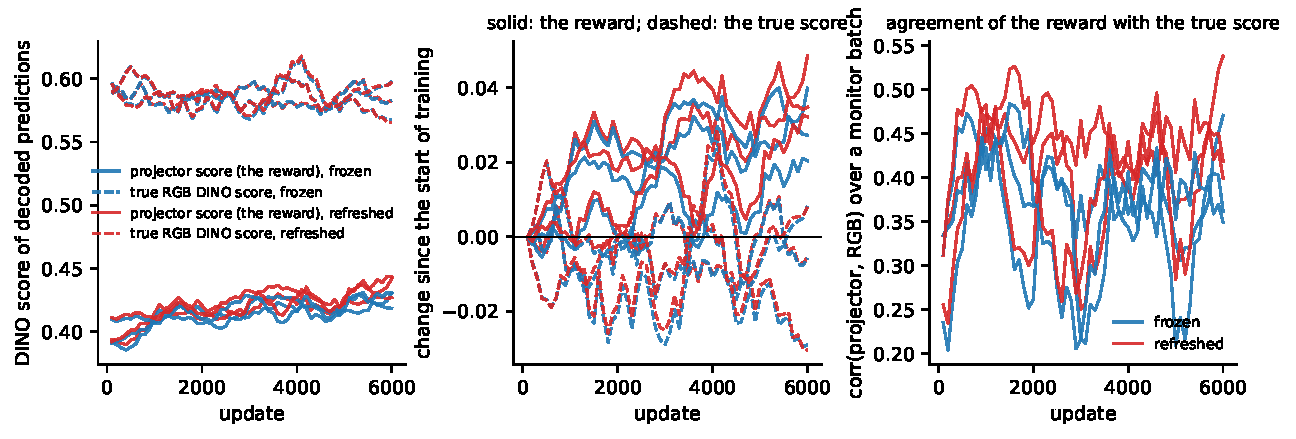
\includegraphics[width=\textwidth]{figs/reward_monitor.pdf}
\caption{The hacking monitor of the six reward runs. Left: projector score (solid) and true RGB score (dashed) of the same decoded predictions over training. Middle: their change since update 100. Right: correlation between the two over each monitor batch. The reward rises in every run; the RGB score does not follow.}
\label{fig:reward}
\end{figure}

Three things happened, in every seed of both arms. The reward went up: the projector score of the decoded predictions rose by 0.02 to 0.04, and the mean reward seen by the optimizer from 0.385 to 0.435 (frozen) and 0.447 (refreshed). The true score did not follow: the RGB DINO score of the same predictions moved by $-0.024$, $-0.006$, $0.000$ (frozen) and $-0.005$, $-0.026$, $-0.001$ (refreshed) per seed, never up. And the benchmarks did not move: after averaging, the frozen-projector arm is $0.0026\pm0.0050$ below argmax and the refreshed arm $0.0003\pm0.0075$ above it on CompBench, with GenEval2 at 24.2 and 24.0 against 23.7, all within seed spread; the refreshed arm is $0.003\pm0.003$ above the frozen one, a consistent sign below resolution.  The refresh did what it could: the correlation between projector and RGB scores over the monitor batches rose from 0.33 to 0.41 (against 0.36 for the frozen projector) but its fitting loss on the student's predictions stayed near 1.0 throughout, so four steps on 32 latents every 100 updates never caught up with the moving prediction distribution. The pattern, a rising proxy with a flat or falling target and no benchmark change, is the signature of a student optimising the scorer rather than what the scorer measures. The projector is a scorer of the frozen teacher's candidates; as a reward on the student's own predictions, at a fifth of the gradient budget, it is inert on alignment and fidelity and is not adopted. Making it a usable reward would need a projector trained on student predictions at the supervised noise levels, with far more of them than a training loop yields cheaply, and a reward that is checked against the RGB score throughout; that is a separate study.

\subsection{What the evidence supports}
The practical choice is settled: argmax selection, stored once, is the best rule tested and the cheapest. Exact soft weighting at $T\le0.08$ is not detectably better and costs 2.3 times the compute; softer rules and uniform weighting are worse or level with random. The explanation of why per-visit resampling underperforms is only partly settled. Its raw-checkpoint deficit is largely final-iterate noise, which checkpoint averaging removes; the remainder is of the size the clipping and second-moment effects measured above can produce, and the fixed-versus-resampled controls do not isolate a persistence effect from optimization variance and candidate coverage in this short-training regime. Separating them would take the same-caption Monte-Carlo estimator (which halves or quarters the sampling variance at single-caption compute) and more seeds; neither was run because the practical conclusion does not depend on it. A decode-free scorer that ranks candidates in latent space is a separate design decision from the selection rule, and Section~\ref{sec:latent} measures it: a small projector on the terminal latent recovers about three quarters of the RGB scorer's selection value offline and in trained students, at no decode cost; since decoding and scoring are under 10\% of the offline selection pipeline (Section~\ref{sec:cost}), its value would be as a scorer inside a training loop rather than as a saving, and Section~\ref{sec:reward} shows that, used as a reward on the student's own predictions, it is optimised without the true score or the benchmarks following.

\clearpage
\section{Ablations}
\label{sec:ablations}
All ablations use the 3k pool, three seeds and the 3k configuration unless stated.

\subsection{Target horizon}
The 1-step Tweedie target is compared with two targets that are closer to the trajectory endpoint: a 2-step chord, which uses $z_{k+2}$ instead of $z_{k+1}$, and the endpoint $z_8$ itself. The 1-step target is the best for both arms and gives the largest selection gain (Table~\ref{tab:horizon}). The 1-step target is 27\% off the endpoint at $k=3$ and 10\% at $k=5$, so it is biased, but its lower variance across visits matters more.

\begin{table}[ht]
\centering
\caption{Target horizon. CompBench / GenEval2, seed means, and the selection gain of DINOv2 patches over random.}
\label{tab:horizon}
\begin{tabular}{l c c c}
\toprule
Target & random & DINOv2 patches & Selection gain (CompBench) \\
\midrule
1-step Tweedie (used) & 0.4584 / 20.73 & 0.4725 / 22.89 & $+0.0140$ \\
2-step chord & 0.4533 / 21.09 & 0.4646 / 21.99 & $+0.0113$ ($p=3\times10^{-6}$) \\
endpoint $z_8$ & 0.4530 / 20.57 & 0.4565 / 20.97 & $+0.0035$ (n.s.) \\
\bottomrule
\end{tabular}
\end{table}

\subsection{Objective: \texorpdfstring{$x_0$}{x0} regression against segment-velocity imitation}
A progressive-distillation-style objective places the student on state $z_k$ and regresses the teacher's velocity chord to $z_{k+1}$ with a mean-squared error. On the 8-step grid, deployed at 4 steps, it is much worse than the $x_0$ objective: random 0.4046 / 17.27 and VQAScore 0.4257 / 20.05 against 0.4584 / 20.73 and 0.4817 / 23.06. The selection gain persists under it ($+0.021$ CompBench), so selection does not depend on the objective, but the objective decides the absolute level.

\subsection{Teacher quality}
\label{sec:k28}
Two stronger teachers were tested with the same captions and seeds: 28 steps at $w=7$ (candidates and training on the 28-step grid, supervised states 10, 14, 18, 22, 26, $\Delta\in\{3,\dots,10\}$), and 16 steps at the model-card guidance $w=4.5$ (the 4-step inference grid nests in the 16-step grid; supervised states 6, 8, 10, 12, 14, $\Delta\in\{2,\dots,6\}$). Both compress the candidate pool a scorer can act on (Table~\ref{tab:scorestats}): the oracle-minus-random VQAScore headroom falls from 0.0905 to 0.0415 (28 steps) and 0.0459 (16 steps), and the fraction of it the DINOv2 patch scorer recovers falls from 43.6\% to 11.0\% at 16 steps (top-1 agreement with the oracle 0.285, chance 0.25). The trained selection gain disappears (Table~\ref{tab:k28}). A stronger teacher on its own is worth about as much on CompBench as scored selection on the 8-step teacher, and the two do not add. Guidance matters separately from step count: 16 steps at $w=4.5$ lifts GenEval2 by 1.3 but CompBench by only 0.004 over the 8-step $w=7$ teacher, while 28 steps at $w=7$ lifts CompBench by 0.021.

\begin{table}[ht]
\centering
\caption{Teacher quality. CompBench / GenEval2, seed means over three seeds, and the paired selection gain within the same teacher.}
\label{tab:k28}
\resizebox{\textwidth}{!}{%
\begin{tabular}{l c c c c}
\toprule
Teacher & DINO headroom recovered & random & DINOv2 patches & Selection gain \\
\midrule
8 steps, $w=7$ & 43.6\% & 0.4584 / 20.73 & 0.4725 / 22.89 & $+0.0140$ / $+2.17$ \\
16 steps, $w=4.5$ & 11.0\% & 0.4624 / 22.02 & 0.4664 / 22.16 & $+0.0040$ ($p=0.07$) / $+0.14$ ($p=0.81$) \\
28 steps, $w=7$ & -- & 0.4797 / 23.06 & 0.4801 / 22.25 & $+0.0004$ ($p=0.87$) / $-0.81$ ($p=0.18$) \\
\bottomrule
\end{tabular}}
\end{table}

Per teacher forward pass this is not a cost win for selection either: four 8-step candidates cost 32 passes per caption, one 28-step sample costs 28.

\subsection{Regression onto the reference photograph}
The reference photograph is the one sample we have from the distribution every scorer points at, so it was tested as a second regression target. On each update the photograph's latent is noised along its own straight path to two random supervised states, and the student's clean-latent estimate there is regressed onto the photograph latent with the same pseudo-Huber loss, added with weight $\lambda=0.2$. On the 16-step teacher, three seeds, this term hurts both arms on both metrics: random $0.4624\to0.4281$ CompBench ($-0.034$, $p=10^{-43}$, worst on UniDet at $-0.052$) and $22.02\to20.67$ GenEval2; DINOv2 patches $0.4664\to0.4407$ ($-0.022$) and $22.16\to20.32$. A single photograph per caption is a far noisier target than the teacher's trajectory, and it pulls the student off the trajectory it must reproduce at inference. The photograph is used for scoring only.

\subsection{Evolving teacher}
\label{sec:ema}
The frozen teacher never moves toward the high-score region; selection only filters what it produces. A self-distillation variant was therefore tested in which the teacher is an exponential moving average of the student. On every update the EMA teacher rolls out four fresh-seed candidates at $w=1$, the DINOv2 patch scorer ranks them against the reference photograph on the fly, and the winner's EMA trajectory provides the targets. Runs start from the 118k averaged patch student (0.4865 / 22.05), use the 3k pool, 6,000 updates and one seed, and are compared with the same student continued against the frozen teacher (Table~\ref{tab:ema}). Both the student and its EMA copy are evaluated.

\begin{table}[ht]
\centering
\caption{Evolving (EMA) teacher, seed 0, 6,000 updates from the 118k patch student. CompBench / GenEval2 of the raw student and of its EMA weights. $\bar S$ is the mean DINOv2 patch score of the teacher's fresh candidates at the end of training (0.60 at the start), $H$ their normalised selection entropy at $T=0.02$ (0.75 at the start).}
\label{tab:ema}
\resizebox{\textwidth}{!}{%
\begin{tabular}{l l c c c c}
\toprule
Teacher & Selection & raw student & EMA weights & $\bar S$ at end & $H$ at end \\
\midrule
frozen (control) & DINOv2 patches, cached & 0.4779 / 19.96 & 0.4847 / 20.68 & -- & -- \\
EMA, decay 0.999 & DINOv2 patches, online & 0.1655 / 0.88 & 0.1789 / 2.09 & 0.03 & 0.93 \\
EMA, decay 0.999 & random & 0.1546 / 1.00 & 0.1667 / 1.52 & 0.03 & 0.93 \\
EMA, decay 0.999, frozen anchor 50\% & DINOv2 patches, online & 0.2095 / 6.28 & 0.2250 / 8.96 & 0.05 & -- \\
EMA, decay 0.9999 & DINOv2 patches, online & 0.4385 / 18.04 & \textbf{0.4936 / 22.33} & 0.62 & 0.75 \\
EMA, decay 0.9999 & random & 0.4296 / 18.51 & 0.4917 / 22.03 & 0.61 & -- \\
\bottomrule
\end{tabular}}
\end{table}

A fast-tracking teacher (decay 0.999) collapses with or without selection and with a 50\% frozen anchor: the candidates' score falls from 0.60 to 0.03 and their selection entropy rises from 0.75 to 0.93, so the scorer can no longer tell them apart, while the training loss falls and the student's samples turn into texture noise. The entropy of the online scores is an early warning of this collapse, visible thousands of updates before any image metric is computed. A slow teacher (decay 0.9999) is inert over 6,000 updates: the candidate score stays at 0.60 to 0.62, and selection within the slow loop is worth $+0.002$ CompBench and $+0.3$ GenEval2 against random ($p>0.5$). Its EMA weights end 0.009 above the frozen-teacher control ($p=0.01$), which is the effect of weight averaging, not of the moving teacher. Continuing the 118k student on the 3k pool with the frozen teacher lowers it (0.4865 to 0.4847), so the small pool is not a source of further gain either. The frozen teacher is kept.

\subsection{Reference photograph aspect handling}
Rescoring the 3k pool with the reference centre-cropped then resized, or resized then cropped, changes the top-1 pick on 12.2\% and 11.8\% of captions and lowers the recovered headroom from 43.6\% to 41.0\% and 40.9\%. Cropping loses captioned objects at the edges, and mean-pooled patches tolerate the distortion of squashing. Squashing is therefore a design choice, not an oversight.

\subsection{Patch mean against CLS token}
The two DINOv2 readouts are the same model, the same decode, the same reference and the same normalisation; only the token summary differs. Offline, the patch mean recovers 43.6\% of headroom against 39.9\% for CLS. Trained, the patch arm is ahead by $+0.0104$ CompBench on identical prompts, positive on all three seeds, while the CLS arm's gain over random has an interval that includes zero. The CLS token is a global summary of what kind of image this is; the patch mean keeps object and layout structure, which is what compositional prompts test.

\clearpage
\section{Qualitative examples}
\label{sec:qual}
Figures~\ref{fig:qual_cb} and~\ref{fig:qual_ge} show prompts on which the scored student differs most from the random-selection student, chosen by the rule stated on each figure: the eight largest per-prompt margins, at most two per CompBench category, seed 0 of each arm, identical initial noise across all columns. They are cherry-picked by construction and show what the gain looks like where it is large, not typical behaviour. On CompBench the scored student wins 366 prompts, loses 229 and ties 1,803 within 0.1; on GenEval2 it wins 169, loses 140 and ties 491 of 800, and both students score below 0.05 on 27\% of the prompts. The columns also show the base model at 4 steps with and without guidance, which fails, and the 28-step teacher, which the students approach. The recurring pattern in the wins is an object that the random-selection student drops or merges (the second object of a two-object prompt, the count of a numeracy prompt) and that the scored student renders, together with cleaner colour and material binding.

\begin{figure}[p]
\centering
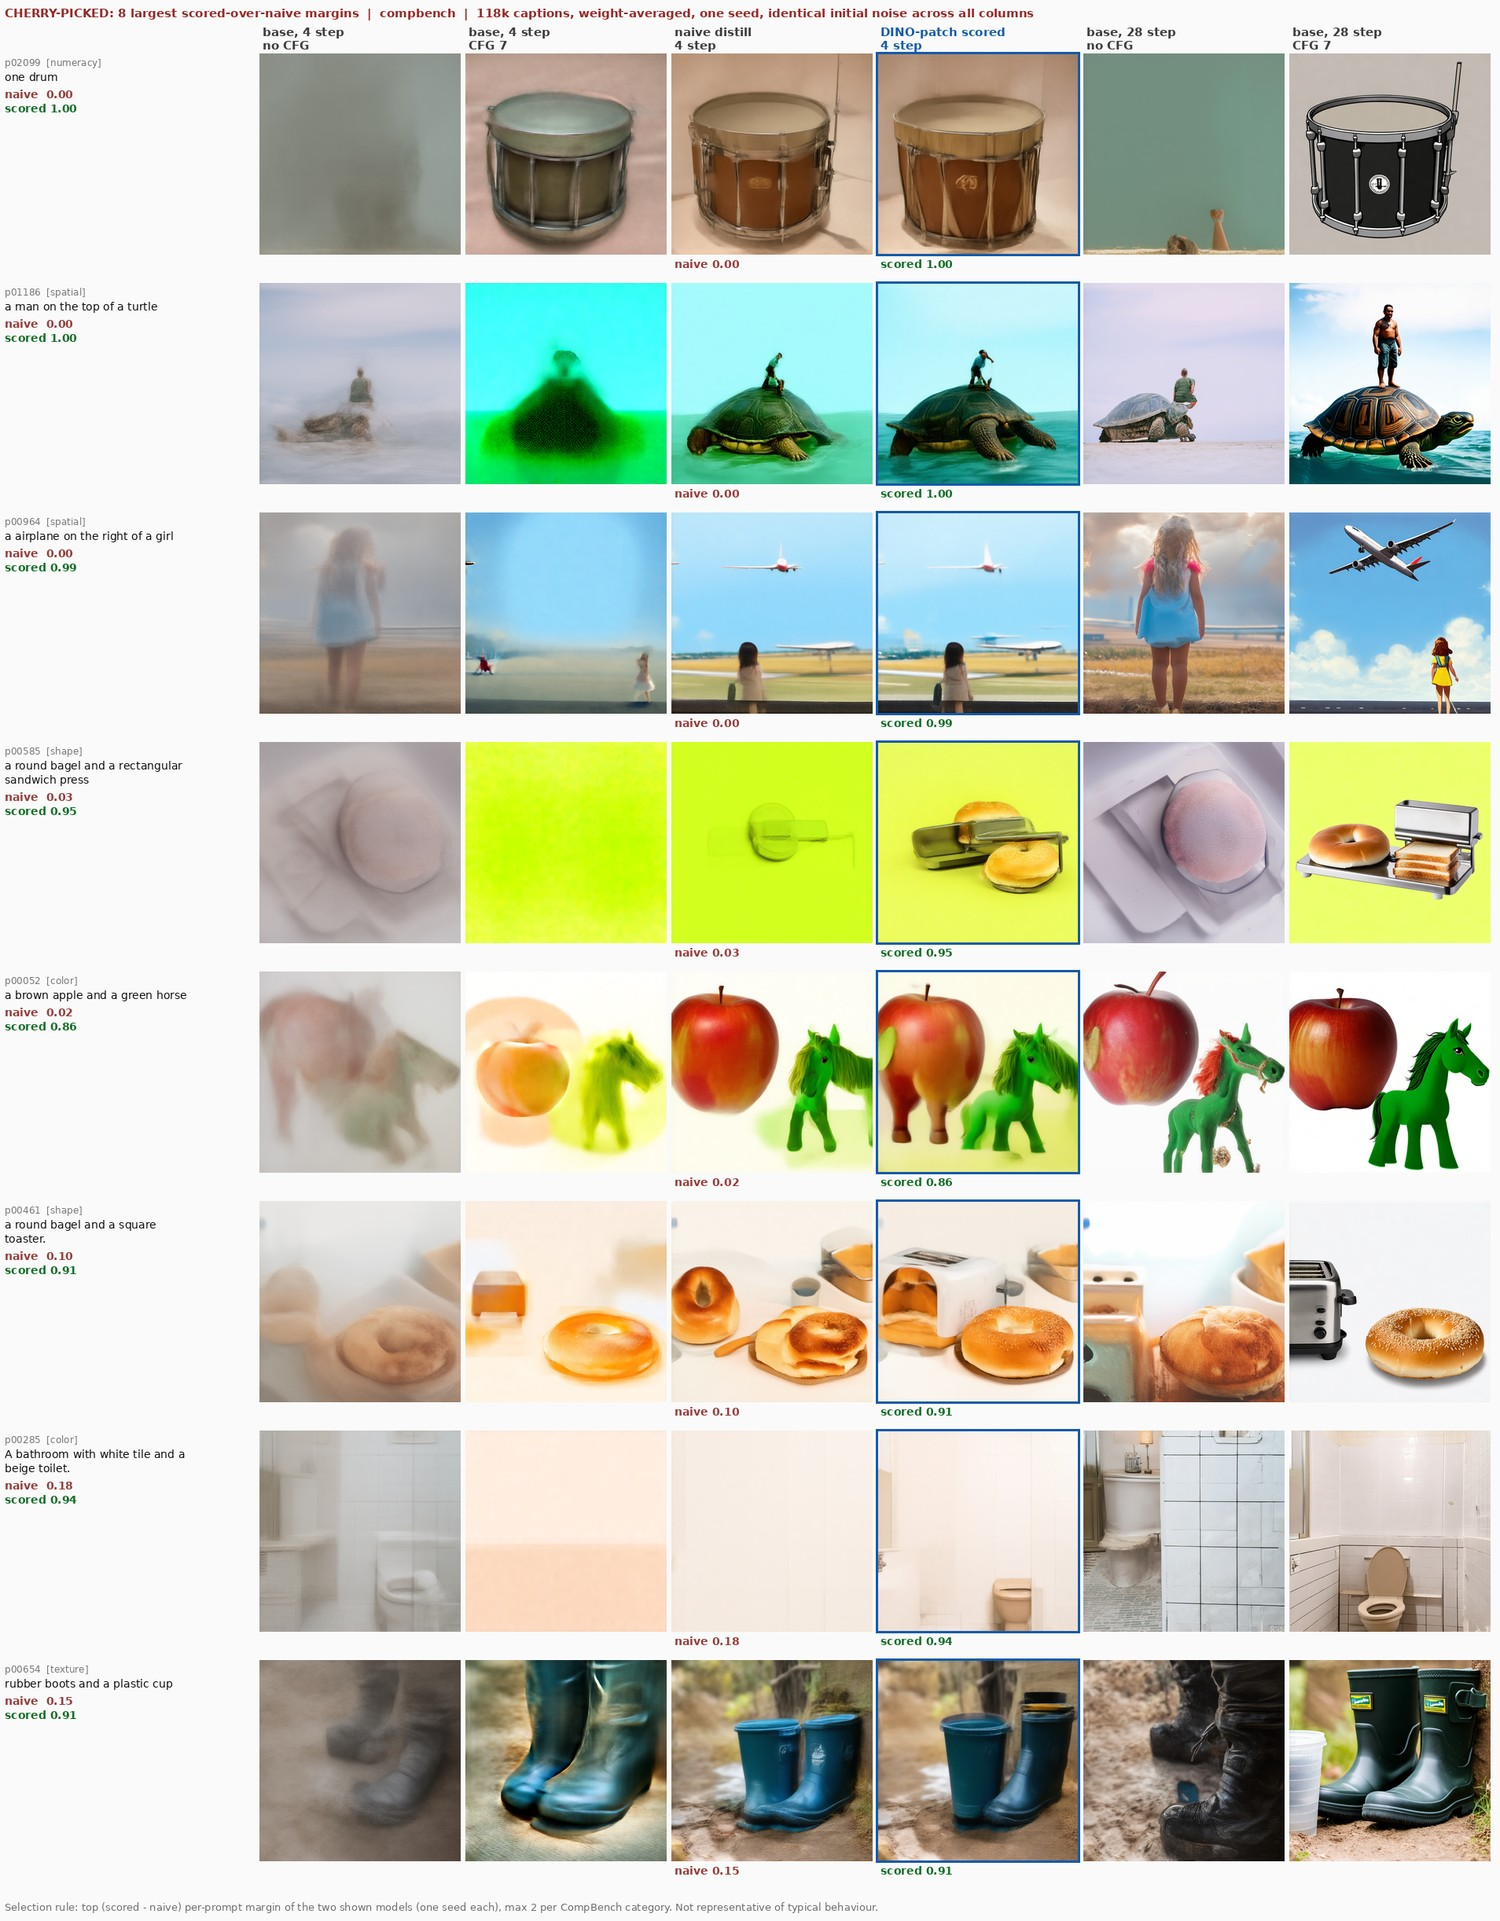
\includegraphics[width=\textwidth]{figs/qual_compbench.jpg}
\caption{T2I-CompBench prompts with the largest scored-over-random margins at 118k. Columns: base model at 4 steps without and with guidance, random-selection student, DINOv2 patch student (framed), base model at 28 steps without and with guidance. Per-prompt scores under each student.}
\label{fig:qual_cb}
\end{figure}

\begin{figure}[p]
\centering
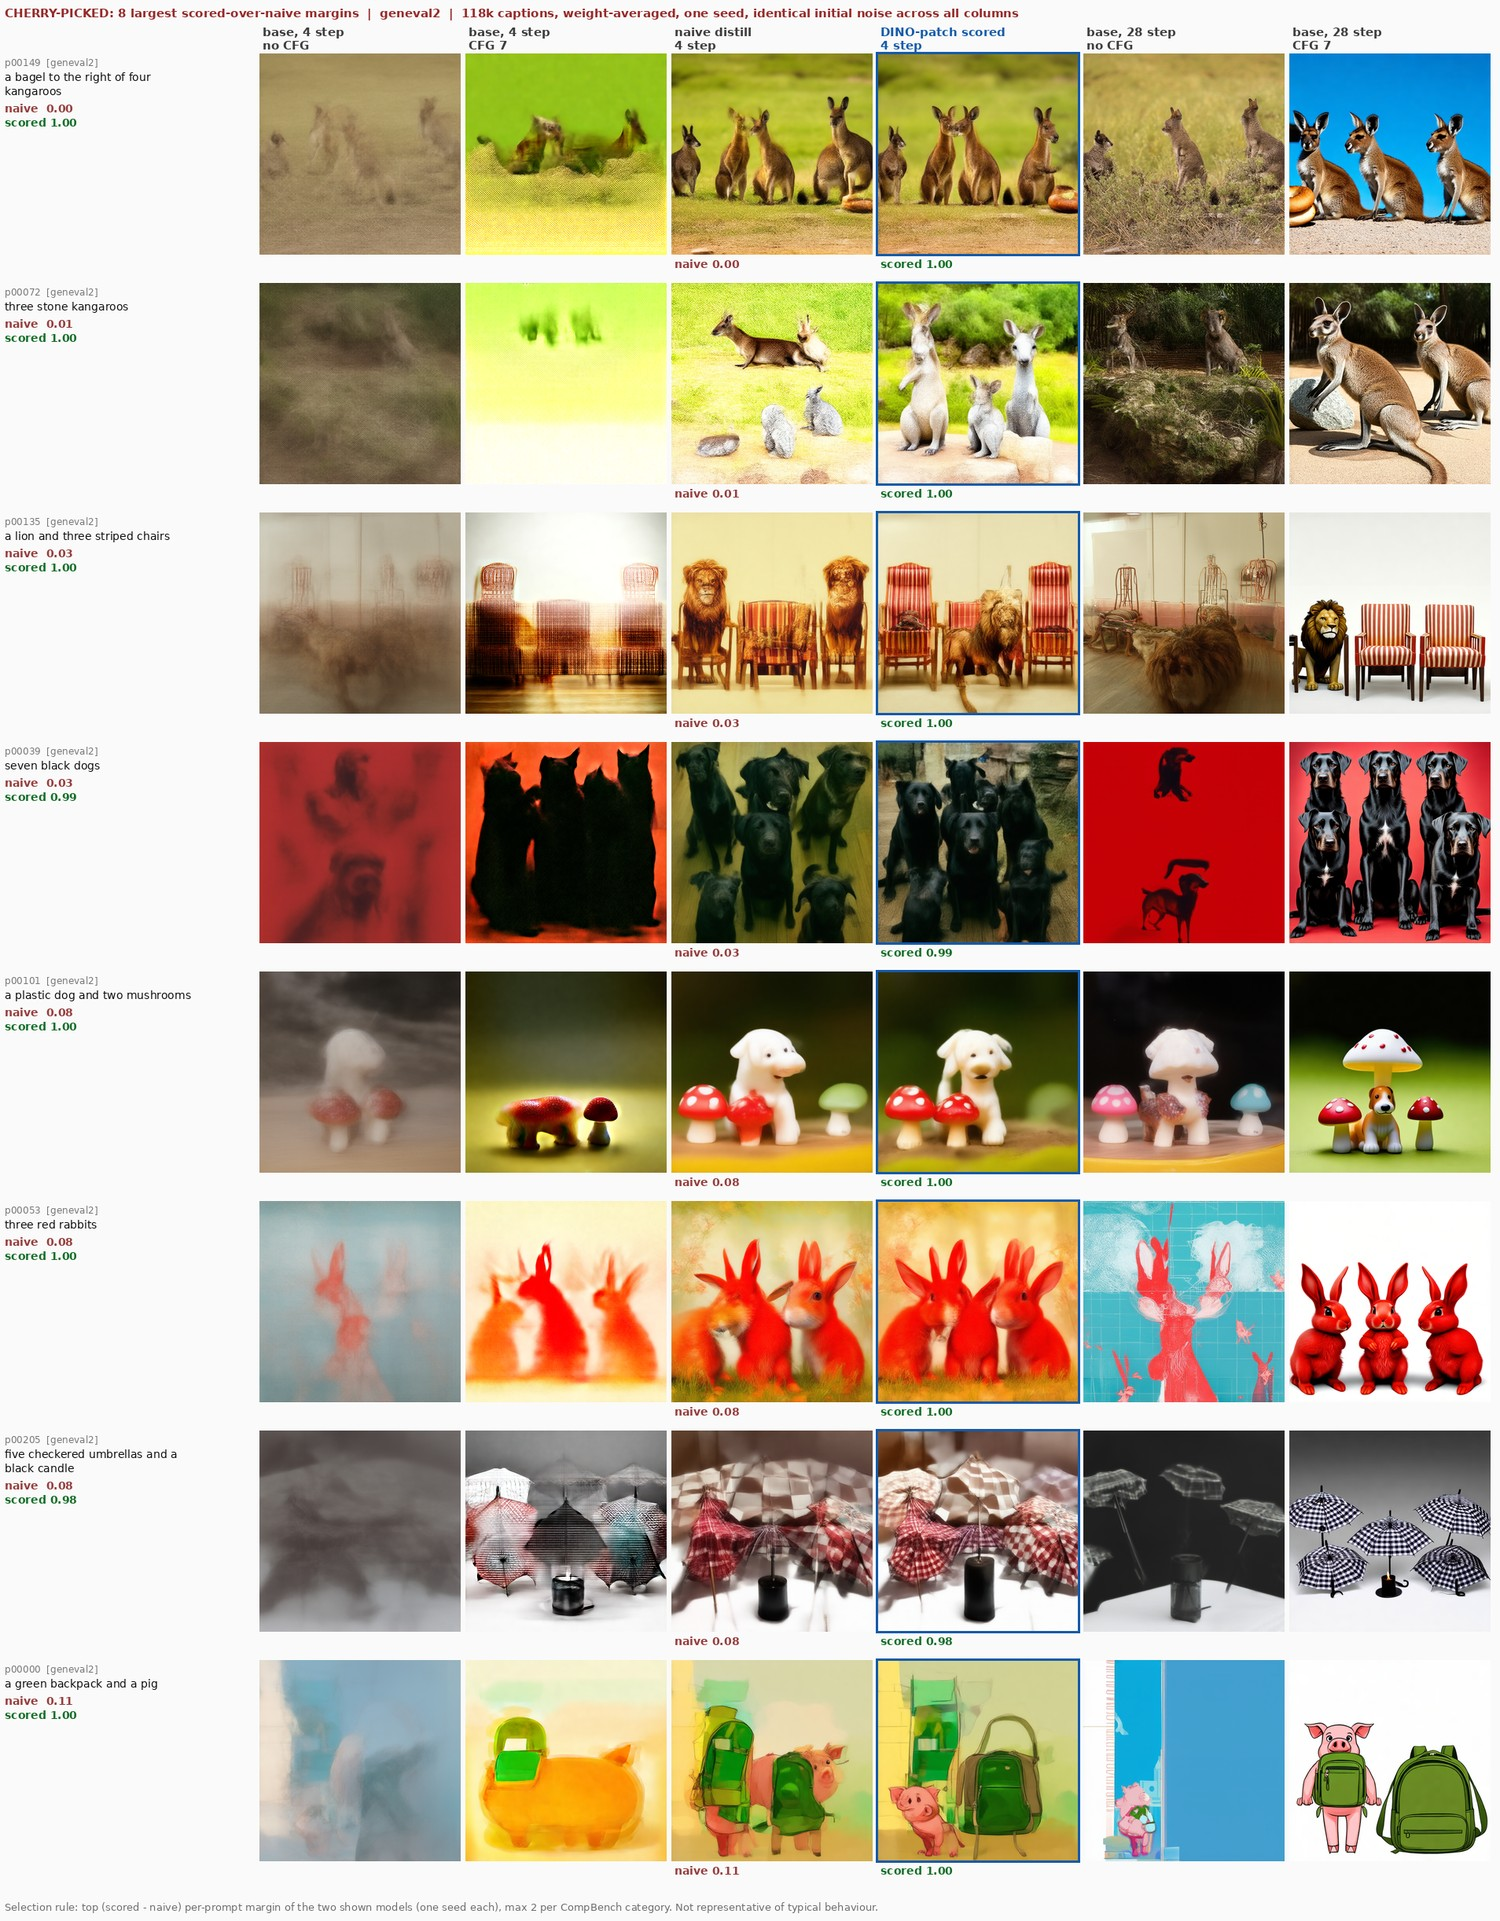
\includegraphics[width=\textwidth]{figs/qual_geneval2.jpg}
\caption{GenEval2 prompts with the largest scored-over-random margins at 118k, same layout as Figure~\ref{fig:qual_cb}.}
\label{fig:qual_ge}
\end{figure}

\clearpage
\section{Cost}
\label{sec:cost}
Per training caption the candidate pool costs 64 teacher forward passes (4 candidates, 8 steps, two guidance branches), four VAE decodes and five DINOv2 forward passes. Measured on one H100 at $512\times512$, generation takes 789 ms per caption, the four decodes 61 ms, DINOv2 scoring 32 ms, CLIP-I 48 ms and VQAScore 280 ms. End to end, DINOv2 selection costs 0.95 s per caption and VQAScore selection 1.19 s; candidate generation dominates and no scorer avoids it. Training costs 16 teacher passes and five student forward-backward passes per caption. A 3k run takes 1.6 hours on one H200; the 118k run takes 12.5 hours on four H200s. The DINOv2 scorer needs no text model and no large VLM at selection time, which is its practical advantage over VQAScore, ImageReward and PickScore. The exact Boltzmann arm of Section~\ref{sec:selrule}, which rolls out and trains on all four candidates, takes 2.6 s per update against 1.15 s for the single-candidate trainer (3.5 h against 1.2 h for a 3k run) for no detected gain over argmax. The latent scorer of Section~\ref{sec:latent} removes the decode and the DINO pass on the candidate (93 ms of the 950 ms per caption) at the price of a 24k-caption latent set (about 7 GPU-hours to generate) and a five-minute projector training.

\section{Design choices}
\begin{itemize}
\item \textbf{Fixed teacher targets, no EMA.} Every target is a function of the frozen teacher's trajectory. There is no bootstrapping and no target drift. Consistency models use an EMA or stop-gradient student copy; we do not.
\item \textbf{Hard selection, stored once.} One candidate per caption, chosen offline. The trainer rolls out one trajectory per caption for every arm, so compute is identical across arms. Exact Boltzmann weighting of all four candidates is not detectably better than argmax at 2.3 times the cost, and the one-sample estimator of the same objective matches it after checkpoint averaging (Section~\ref{sec:selrule}). Four candidates are enough; eight add nothing (Section~\ref{sec:n8}).
\item \textbf{Guidance internalised.} The student trains with one conditional pass against guided teacher trajectories and is sampled at $w=1$. This halves the student's inference cost relative to a guided sampler.
\item \textbf{Re-roll instead of store.} Trajectories are re-rolled from integer seeds. The cache holds only seeds, scores and indices.
\item \textbf{Reference photograph squashed to a square.} Cropping discards captioned content; see the aspect ablation.
\item \textbf{Mean-pooled patches, CLS dropped.} The patch mean carries layout; the CLS token does not select well.
\item \textbf{Weight averaging at scale.} The last five checkpoints are averaged because single checkpoints of a long run oscillate by more than the effect.
\item \textbf{One sealed evaluation pool and fixed evaluation seeds.} Every arm and seed is scored on identical prompts and identical noise, so all contrasts are paired.
\end{itemize}

\section{Limitations}
\begin{itemize}
\item \textbf{The scorer needs a reference photograph.} DINOv2 selection, and the latent scorer distilled from it, are only possible where each caption has a real image. They cannot be applied to synthetic prompt sets without one.
\item \textbf{Grids do not nest.} The 4-step inference grid shares only its endpoints with the 8-step training grid, so the student is deployed at $\sigma=0.858$ and $0.602$, which it never saw as training inputs, and is never trained at $\sigma=0.009$ (the last step is scaled by 0.009 and is immaterial). Grids with $K\in\{7,10,13,16,\dots\}$ nest exactly; this was not used here.
\item \textbf{Duplicate student inputs.} With five independent $\Delta_k$ draws, 81\% of updates contain at least one repeated input state and the expected number of distinct inputs is 3.9 of 5. This does not change the objective, only its variance, and wastes about 22\% of student passes.
\item \textbf{Seeds.} Every headline number is three training seeds. The single-seed contrasts (the VQAScore arm at 118k, the batch-size row, the evolving-teacher runs) are marked as such and resolve about 0.01 CompBench.
\item \textbf{Selection-rule contrasts are three-seed contrasts.} They resolve about 0.01 CompBench at the level of training runs. ``No detected improvement'' over argmax is the claim; equivalence is not.
\item \textbf{Checkpoint averaging is part of the method at scale.} Without it the 118k gap is $+0.007$ instead of $+0.0175$. Averaging is applied identically to every arm, but the reported 118k numbers are for averaged weights.
\item \textbf{Selection gain depends on candidate variance.} With a 28-step or a 16-step $w=4.5$ teacher the within-caption score spread halves and the gain vanishes. Scored selection is a fixed-teacher gain, not a substitute for teacher quality.
\item \textbf{VQAScore is circular.} Its gains share a model family with the BLIP-VQA categories of CompBench and the VLM judge of GenEval2. It is included as a reference, not as the proposed method.
\item \textbf{Metric properties.} GenEval2's geometric mean rewards partial credit, and CompBench 2D-spatial has dead prompts (Section~\ref{sec:metricprops}). Both are constant across arms and do not reorder students, but they limit what absolute numbers mean.
\end{itemize}

\section{Reproducibility}
The release code is the \texttt{scored-consistency-distillation} branch of the project repository. It contains the pool builder, the candidate scorer, the trainer with the \texttt{random}, \texttt{dino\_patch}, \texttt{boltzmann}, \texttt{boltzmann\_sample}, \texttt{boltzmann\_frozen}, \texttt{boltzmann\_mc} and \texttt{uniform\_visit} selectors, gradient accumulation, the gradient diagnostic, the latent scorer (latent generation, projector training, the \texttt{latent} selector, the projector reward with its monitor and refresh), the checkpoint averager, the evaluation scripts (CompBench with the one- and ten-image protocols, GenEval2, COCO VQAScore, FID, reference CMMD, precision and recall), the figure script and the LSF launch scripts. The release trainer was verified to be bit-identical to the experimental trainer that produced every number in this document, on all 909 parameter tensors after six optimizer updates under deterministic kernels, for every selector and for gradient accumulation, with an original-versus-original control at exactly zero. Every evaluation writes a pinned record with evaluator commits, package versions, pool hashes and the checkpoint hash, and fails hard on missing images. Training runs log per-state losses, selection statistics, throughput, sample grids and a source snapshot to Weights \& Biases.

\begin{thebibliography}{9}
\bibitem{sd3} P. Esser et al. Scaling rectified flow transformers for high-resolution image synthesis. ICML 2024.
\bibitem{cm} Y. Song, P. Dhariwal, M. Chen, I. Sutskever. Consistency models. ICML 2023.
\bibitem{ict} Y. Song, P. Dhariwal. Improved techniques for training consistency models. ICLR 2024.
\bibitem{dinov2} M. Oquab et al. DINOv2: learning robust visual features without supervision. TMLR 2024.
\bibitem{vqascore} Z. Lin et al. Evaluating text-to-visual generation with image-to-text generation. ECCV 2024.
\bibitem{compbench} K. Huang et al. T2I-CompBench: a comprehensive benchmark for open-world compositional text-to-image generation. NeurIPS 2023.
\bibitem{geneval2} GenEval2: compositional text-to-image evaluation with atom-level VLM judging. 2025.
\bibitem{cmmd} S. Jayasumana et al. Rethinking FID: towards a better evaluation metric for image generation. CVPR 2024.
\bibitem{imagereward} J. Xu et al. ImageReward: learning and evaluating human preferences for text-to-image generation. NeurIPS 2023.
\bibitem{pickscore} Y. Kirstain et al. Pick-a-Pic: an open dataset of user preferences for text-to-image generation. NeurIPS 2023.
\end{thebibliography}

\end{document}
